% !TEX encoding = UTF-8
% !TEX TS-program = pdflatex
% !TEX root = ../tesi.tex

%**************************************************************
\chapter{Resoconto dello stage}
\label{cap:resoconto-stage}
%**************************************************************

\intro{In questo capitolo verranno descritte le attività svolte durante lo stage. Per ogni attività si cercherà di descrivere il problema affrontato, le scelte effettuate ed i test svolti.}\\

%\section{Pianificazione}
%La prima attività svolta, in realtà ancora prima dell'inizio dello stage stesso, è stata quella di pianificare il lavoro da svolgere. Tale %pianificazione è stata concordata tra il tutor aziendale e il sottoscritto, ed è esposta nella sezione \ref{sec:vincoli-temporali} a pagina %\pageref{sec:vincoli-temporali} di questo documento.\\
%Tale pianificazione, però, è stata "aggiustata" (ma mai stravolta) in base a quanto svolto settimana per settimana, decidendo di dedicare più o meno ore ad una determinata attività.\\
%Al termine di ogni settimana, periodo coincidente con il raggiungimento di un obiettivo, infine, è stato deciso che avrei dovuto redarre una %breve relazione, con lo scopo di documentare il lavoro svolto. Tali relazioni, inoltre, sono servite come materiale ausiliario per la %presentazione delle nuove funzionalità sviluppate al proponente. Infine, terminati tutti gli obiettivi e in caso di approvazione da parte del %tutor e del proponente, avrei dovuto trasferire il lavoro svolto dall'ambiente di sviluppo a quello di produzione.

\section{Scelte tecnologiche e strumenti utilizzati}
A livello tecnologico, dato che il \bookingEngine\hphantom{i}è basato sullo stack che in azienda viene chiamato \gls{wisp}, sono stato obbligato ad utilizzare \textit{PHP} su \gls{framework} \textit{Codeigniter} per la parte \textit{backend}, \textit{HTML5}, \textit{CSS3}, \textit{Javascript} (principalmente utilizzando \gls{jquery}) per quanto riguarda il \textit{frontend}. Infine, per la comunicazione tra \textit{backend} e \textit{frontend} ho adoperato richieste \gls{ajax} con \gls{json} come formato per lo scambio di dati. Come ambiente di sviluppo ho deciso di usare \textit{Visual Studio Code} per via della sua semplicità e possibilità di personalizzazione. Infine, tutto il lavoro che ho svolto è stato sottoposto a versionamento utilizzando il server \textit{Git} dell'azienda. 

\section{Funzionamento e struttura del \bookingEngine}
Appena iniziato lo stage, mi sono subito dedicato all'analisi della struttura di CrociereRegalo, grazie anche (soprattutto all'inizio) all'aiuto del mio tutor. 
\subsection{Funzionalità}
CrociereRegalo è un motore di ricerca di crociere. Permette di trovare una determinata crociera utilizzando dei filtri di ricerca per area geografica (ad esempio Caraibi, Mediterraneo, Nord Europa), per data di partenza con granularità mensile (ad esempio Settembre 2018), per intervalli di durata (da 1-6, 7-8, 9-12 o più di 12 giorni) e per compagnia di crociera (ad esempio MSC Crociere). Per capire bene il suo funzionamento è stato necessario apprendere alcuni termini tecnici affini all'ambiente croceristico, come:
\begin{itemize}
	\item \textbf{Itinerario}: definisce il percorso che fa una crociera (ad esempio "Barcellona, Ajaccio, Civitavecchia, Barcellona"). Nell'arco di un periodo di tempo vi possono essere molteplici crociere percorrenti un singolo itinerario. Ogni itinerario è identificato da un codice che lo contraddistingue univocamente, e la durata dell'itinerario è una proprietà intrinseca (ovvero, all'interno di una compagnia di crociera, non esistono due itinerari che svolgono lo stesso percorso mettendoci tempi diversi). Ciascun itinerario ha 0 o più partenze nell'arco di un anno;
	\item \textbf{Cabina}: una stanza di una nave da crociera. Esistono varie categorie di cabina, differenziate in base alla grandezza, al posizionamento (ad esempio le cabine interne alla nave, senza quindi finestre, che sono quelle più economiche). Quando si effettua una prenotazione, non viene prenotato un posto letto ma viene prenotata un'intera cabina;
	\item \textbf{Opzione}: consiste nel blocco del prezzo di una cabina per un periodo di tempo che varia in base al fornitore, ma che di solito si attesta tra le 24 e le 72 ore. Tale prezzo infatti, analogamente per quanto avviene con i biglietti aerei, aumenta all'aumentare delle prenotazioni (quindi al passare del tempo).

\end{itemize}
CrociereRegalo permette di selezionare un itinerario, vederne le partenze, categorie di cabina disponibili e prezzi e poi prenotare od opzionare una cabina. 

\subsection{OTA e DataExchange}
Mi è stato spiegato che il \bookingEngine, in realtà, era spezzato in due parti dipendenti l'una dall'altra: \textbf{OTA} (disponibile all'indirizzo \cite{site:crociereregalo}) e \textbf{DataExchange} (disponibile all'indirizzo \cite{site:dataexchange}). L'idea alla base di questa divisione è che la parte \textit{OTA} rappresenti il sito web vero e proprio, con il quale l'internauta si affaccia, mentre la parte \textit{DataExchange} serva per l'interazione tra \textit{OTA} e \glspl{webservice} dei vari fornitori (dove per fornitori si intendono le varie compagnie di crociera). 

\subsection{Interazione tra OTA e DataExchange}
\textit{OTA} e \textit{DataExchange} sono dipendenti l'uno dall'altro, ma hanno due database separati. Questo, fondamentalmente, avviene perchè i dati provenienti da i vari fornitori hanno formati diversi, che devono quindi essere uniformati per poter essere processati secondo una logica più indipendente possibile. Il compito del \textit{DataExchange} è proprio questo: interrogare i \glspl{webservice} dei vari fornitori, ricevere i dati, elaborarli, uniformarli e passarli ad \textit{OTA}.\\
Vi sono due possibili interazioni tra \textit{OTA} e \textit{DataExchange}
\begin{itemize}
	\item Interazione \textbf{schedulata} (illustrata in Figura \ref{figura:integrazione-schedulata}), che avviene circa 3 volte al giorno, il cui compito è sincronizzare i cataloghi (chiamati anche \textit{flatfile}) dei vari fornitori per rendere disponibili le (eventuali) modifiche alla parte \textit{OTA} del \bookingEngine. \\Quando un visitatore del sito CrociereRegalo cerca una crociera, tale ricerca avviene interrogando i cataloghi presenti nel database della parte \textit{OTA}, senza quindi interrogare i \glspl{webservice} delle compagnie di crociera (per motivi di prestazione dovuti all'ingente mole di dati da elaborare). I cataloghi, quindi, vengono scaricati nel DataExchange, elaborati (uniformati) e poi sincronizzati con il database di OTA; la procedura di sincronizzazione viene chiamata \textbf{Integrazione}. L'integrazione avviene attraverso l'invocazione (grazie allo scheduler di \textit{Windows Server}) che, grazie ad una chiamata \textit{HTTP} ad una particolare pagina del DataExchange, invoca la procedura di integrazione dati.
	\begin{figure}[!h] 
		\centering 
		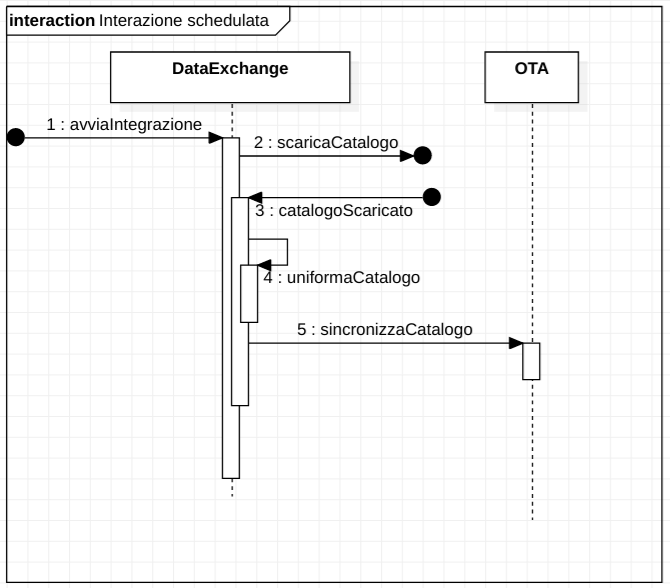
\includegraphics[width=.75\columnwidth]{attivita/interazione_schedulata} 
		\caption{Schema dell'integrazione schedulata DataExchange-OTA.}
		\label{figura:integrazione-schedulata}
	\end{figure}
	\item Interazione \textbf{real-time} (rappresentata in Figura \ref{figura:integrazione-realtime}), che avviene durante tutto il flusso di prenotazione di una cabina (che analizzerò in seguito). Tale flusso deve per forza disporre di dati aggiornati in tempo reale, altrimenti potrebbero verificarsi problemi in fase di prenotazione (come la prenotazione di una cabina non più disponibile). L'interazione in tempo reale avviene attraverso delle chiamate \textit{HTTP} (\gls{ajax}) effettuate nel momento del bisogno dall'\textit{OTA} al \textit{DataExchange}, attraverso lo scambio di dati in formato \gls{json}.
	\begin{figure}[!h] 
		\centering 
		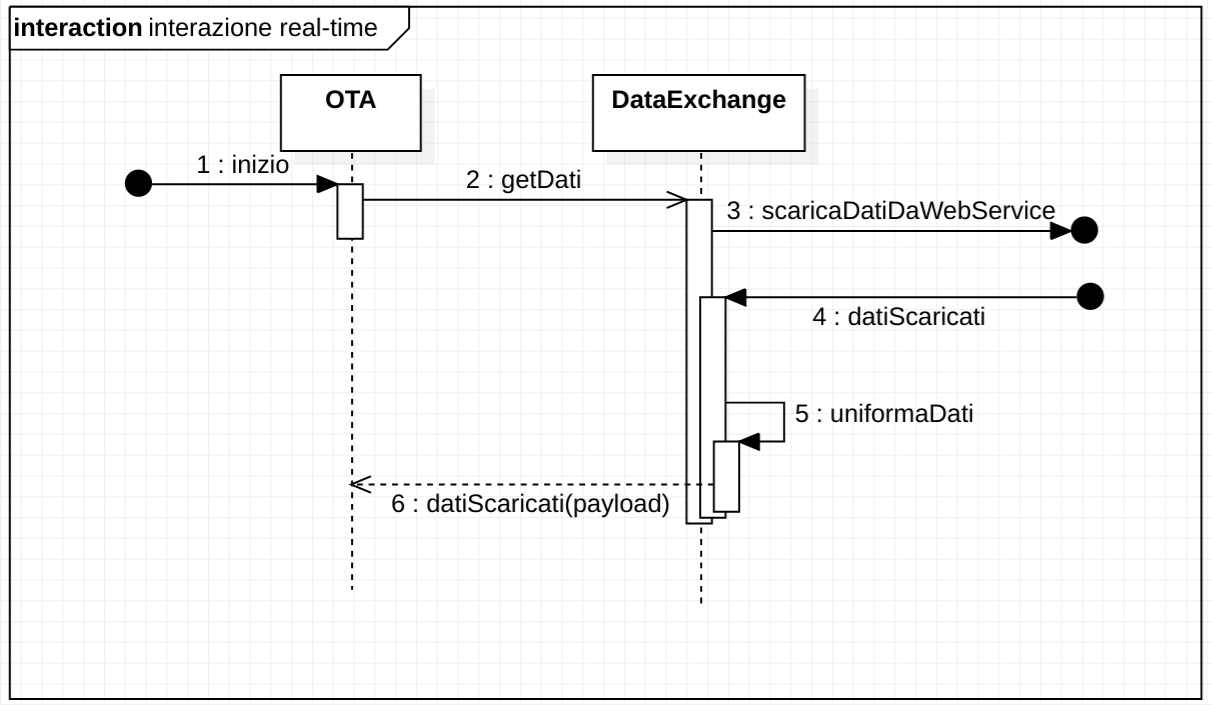
\includegraphics[width=.75\columnwidth]{attivita/interazione_realtime} 
		\caption{Schema dell'integrazione in tempo reale DataExchange-OTA.}
		\label{figura:integrazione-realtime}
	\end{figure}
\end{itemize}

\subsection{Flusso di prenotazione}
\label{section:flusso-prenotazione}
Quando il visitatore, in seguito alla ricerca, apre i dettagli di una partenza, viene data la possibilità di poter avviare la procedura (flusso) di prenotazione, che si avvale dell'interazione real-time tra \textit{OTA} e \textit{DataExchange} si compone nei passaggi illustrati in Figura \ref{figura:flusso-prenotazione}.
	\begin{figure}[!h] 
	\centering 
	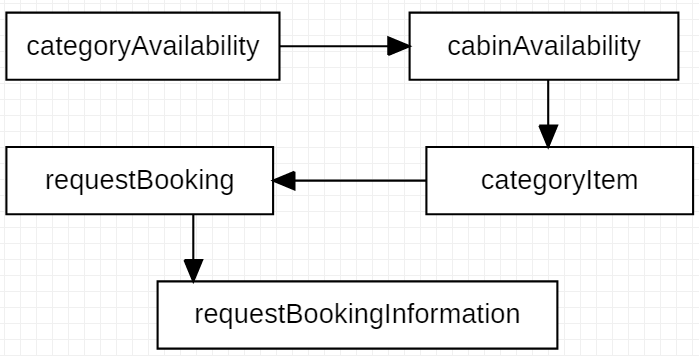
\includegraphics[width=.75\columnwidth]{attivita/flusso_prenotazione} 
	\caption{Schema del flusso di prenotazione}
	\label{figura:flusso-prenotazione}
\end{figure}
Nel dettaglio:
\begin{enumerate}
	\item \textit{categoryAvailability}: vengono elencati i gruppi (categorie) di cabine effettivamente disponibili (o un messaggio di errore in caso non vi siano più posti prenotabili) tenendo conto del numero di passeggeri inseriti (banalmente, se si selezionano 4 passeggeri, vengono mostrati le categorie di cabine nelle quali vi è presente almeno una quadrupla) e dell'età di tali passeggeri (per il calcolo preciso della tariffa, in quanto un minore paga meno di un adulto);
	\item \textit{cabinAvailability}: una volta selezionata una categoria di cabine, vengono mostrate tutte le cabine (una per una) ancora disponibili, raggruppate in base al ponte della nave in cui si trovano;
	\item \textit{categoryItem}: vengono elencati tutti i servizi extra (e relativi prezzi) disponibili in aggiunta a quelli già inclusi nel prezzo della cabina, e viene data la possibilità di selezionarli per aggiungerli alla prenotazione;
	\item \textit{requestPricing}: viene mostrato il prezzo finale (preso dal \gls{webservice} del fornitore) della prenotazione, tenendo conto di quanto selezionato negli step precedenti. Tale prezzo include anche le tasse portuali ed eventuali oneri aggiuntivi;
	\item \textit{requestBooking}: viene effettuata una prenotazione od un'opzione di quanto selezionato negli step del flusso precedenti. Nel caso di prenotazione, viene anche gestito il pagamento (tramite \gls{api} fornite dal consorzio \textit{Triveneto Bassilichi}).
	\item \textit{requestBookingInformation}: viene mostrato il riepilogo di ciò acquistato, con la possibilità di saldare quanto ancora dovuto (nel caso la prenotazione ammetta il versamento di un acconto).
\end{enumerate}

\subsection{Struttura del codice}
\label{section:struttura-codice}
Sia \textit{OTA} che \textit{DataExchange} sono realizzati usando il \gls{framework} \textit{Codeigniter}. Questo implica che applicano a PHP il paradigma \textit{Object-oriented} (orientato agli oggetti) associato al design pattern \gls{mvc}. Entrambi i progetti, dunque, presentano tre tipologie di classi:
\begin{itemize}
	\item \textbf{Model}, che estendono la classe base \textit{CI\_Model}, i quali sono la chiave di accesso ai dati dell'applicazione. Si è deciso di realizzare un \textit{model} per ogni tabella presente nel database;
	\item \textbf{View}, che generano il codice HTML di ogni pagina (o porzione di essa). Alle \textit{view} è possibile passare delle variabili in modo da rendere dinamico il loro contenuto.
	\item \textbf{Controller}, che estendono la classe base \textit{CI\_Controller} e istanziano le \textit{view} popolandole con i dati provenienti dai \textit{model}. La particolarità di queste classi è che i loro metodi pubblici si possono chiamare direttamente tramite URL. Codeigniter, infatti, implementa un meccanismo (grazie al \textit{magic method \_\_call}) per il quale è possibile chiamare un metodo pubblico \textit{a} di una classe controller \textit{C} semplicemente recandosi all'url \textit{nomedelsito.dominio/C/a} (ad esempio \textit{crociereregalo.it/C/a}). Tale meccanismo risulta molto utile nella realizzazione di \gls{api} e nella creazione di \textit{URL} user-friendly (quindi più leggibili)
\end{itemize} 
Codeigniter, inoltre, presenta un modulo personalizzato per interagire con il database, che supporta funzionalità come il \textit{log delle query} (in pratica è possibile sapere l'ultima query eseguita, molto utile in caso di \textit{debug}), meccanismi di \textit{query building} (creazione assitita di query), \textit{query parametrizzate}, gestione delle transazioni ecc.

\section{Ottimizzazione delle performance del database}
\subsection{Il problema}
Il sito CrociereRegalo soffriva di un grande problema: la lentezza di caricamento delle pagine. Tale lentezza era dovuta principalmente all'elevato numero di query complesse presenti in ogni pagina, ciascuna delle quali aveva dei tempi di esecuzione nell'ordine dei secondi che, complessivamente, facevano sì che il tempo di caricamento di alcune pagine (in primis quella di visualizzazione dei risultati di una ricerca) lambisse pericolosamente il minuto.
\subsection{La soluzione trovata}
Dopo un'attenta analisi del database, è emerso che molte tabelle non avevano una corretta struttura. In particolare, su alcune non vi era definita alcuna chiave primaria, mentre in generale non erano presenti chiavi esterne ed indici. Sono quindi state definite chiavi esterne e primarie per tutte le tabelle, mentre per la creazione di indici ci si è affidati all'analisi delle principali query grazie allo strumento \textit{Database Tuning Engine Advisor} integrato nella suite di \textit{SQL Server}. Vengono ora riportati due esempi di analisi svolta e di risultati ottenuti.
\subsubsection{Query di ricerca}

\begin{lstlisting}
SELECT distinct TOP 100 l.Supplier, l.NameIT, l.Description, l.Logo, il.ShipCode,il.SailingLengthDays, il.ItineraryCode, po1.Code as PortoPartenzaCode ,po1.Name as PortoPartenza, po2.Name as PortoArrivo, po2.Code as PortoArrivoCode, min(il.SailingDate) as MinSailingDate, min(p.BestPrice) as BestPrice,it.GraphicsUrl,sp.Name as ShipName 
FROM Cruises_ItineraryList il inner join Cruises_Lines l on il.Supplier= l.Supplier inner join Cruises_Ports po1 on (po1.Code = il.DepartingPort and po1.Supplier = il.Supplier ) inner join Cruises_Ports po2 on (po2.Code = il.EndPort and po2.Supplier = il.Supplier) inner join Cruises_Ship sp on (sp.Supplier=il.Supplier and sp.Code = il.ShipCode) inner join Cruises_Prices p on (p.Supplier=il.Supplier and p.CruiseId = il.CruiseID and p.CruiseCategoryAvailable=1) inner join Cruises_Itinerary it on (it.Supplier=il.Supplier and il.ItineraryCode = it.Code) 
WHERE il.Supplier=1 AND il.AvailabilityStatusCode= 'AV' AND BestPrice > 0 
GROUP By l.Supplier, l.NameIT, l.Description, l.Logo, il.ShipCode,il.SailingLengthDays, il.ItineraryCode, po1.Code, po2.Code, po1.Name, po2.Name , sp.ImgUrl,it.GraphicsUrl,sp.Name order by MinSailingDate,PortoArrivo,ItineraryCode
\end{lstlisting}
Questa è una delle query (la più esterna) che viene usata nel caso di ricerca di un itinerario filtrandolo per fornitore (in questo caso MSC Crociere) i cui esiti vengono utilizzati per creare la schermata presente in Figura \ref{figura:query-1}. Il problema di questa interrogazione, oltre alla lunghezza, è l'elevato numero di JOIN tra tabelle aventi un ingente quantitativo di dati, nello specifico:
\begin{itemize}
	\item Cruises\_Prices: 424 780 righe
	\item Cruises\_ItineraryList: 8 092 righe
	\item Cruises\_Ports: 4 187 righe
	\item Cruises\_Itinerary: 2 985 righe
\end{itemize}
\begin{figure}[!h] 
	\centering 
	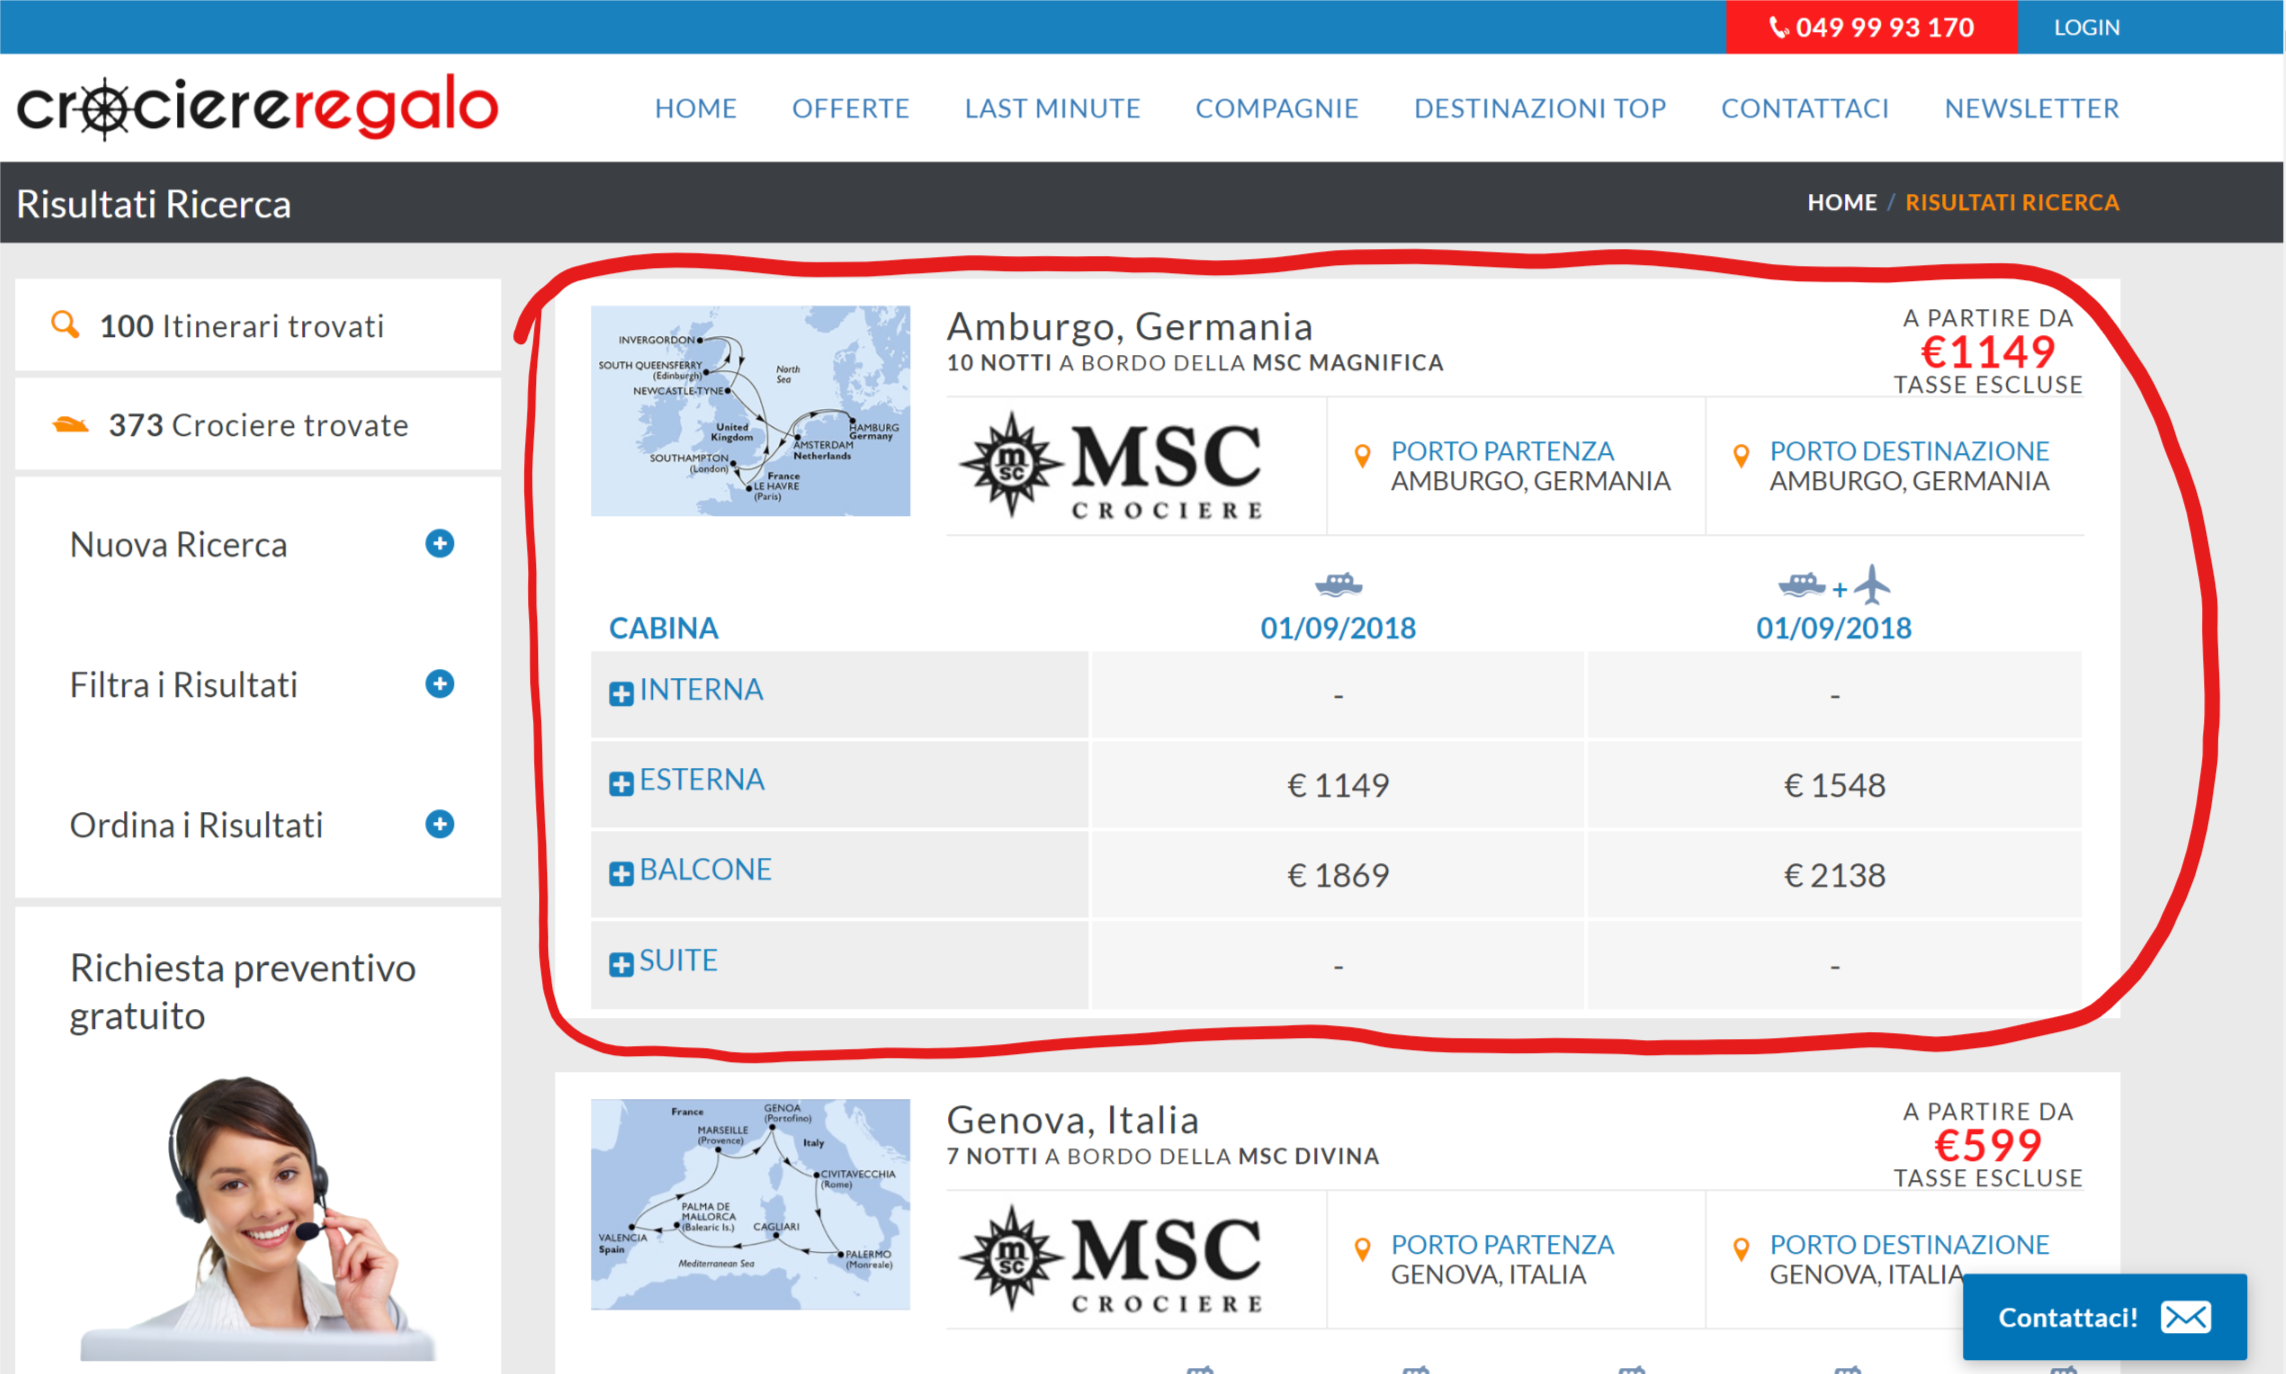
\includegraphics[width=1\columnwidth]{attivita/risultato_ricerca} 
	\caption{Esempio di utilizzo del risultato della query della ricerca.}
	\label{figura:query-1}
\end{figure}
Tali tabelle erano per lo più sprovviste di indici, pertanto le operazioni di JOIN risultavano molto costose. Come risultato si otteneva un tempo di esecuzione, nel server di produzione in assenza di sovraccarichi, variabile tra 23 e 25 secondi. Grazie al tool \textit{Database Tuning Engine Advisor} sono stati creati dei nuovi indici, precisamente su tutte le colonne coinvolte nelle clausole di JOIN. Questo ha portato un ingente riduzione nei tempi di esecuzione della query, che sono arrivati a sfiorare i 2 secondi. Vi è stato, quindi, un miglioramento di ben 21 secondi (circa il 91\%) nel tempo di esecuzione della query e di conseguenza nel \gls{tempodirisposta} della pagina web incaricata di elaborare e visualizzare i risultati della ricerca.\\


\subsubsection{Query dei last minute}
In homepage vi è una sezione che visualizza tutte le offerte \textit{last minute} (ovvero crociere prossime alla partenza aventi ancora posti disponibili a prezzo scontato) presenti nel database, come mostrato in Figura \ref{figura:query-2}. Queste ultime vengono inserite a mano dai dipendenti di \textit{Primarete}, ma sono collegate a crociere effettivamente presenti. La query sottostante restituisce tali offerte.
\begin{figure}[!h] 
	\centering 
	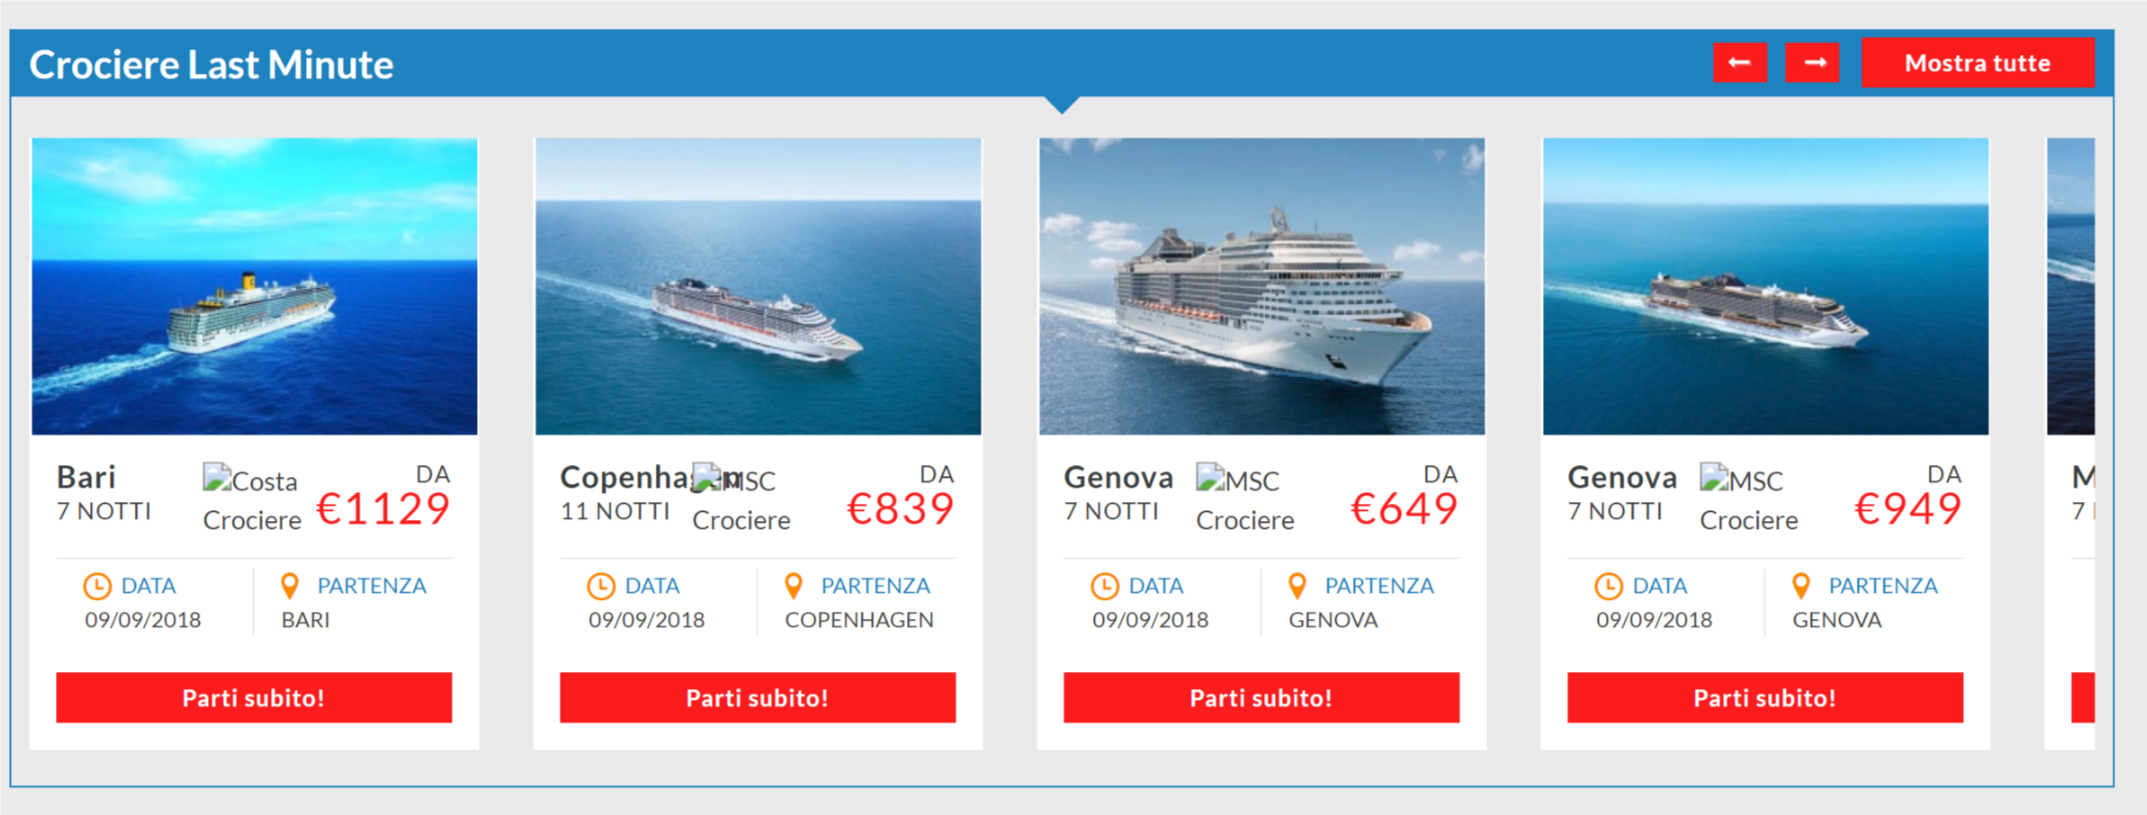
\includegraphics[width=1\columnwidth]{attivita/last_minute} 
	\caption{Esempio di utilizzo del risultato della query dei last minute.}
	\label{figura:query-2}
\end{figure}
\begin{lstlisting}
SELECT distinct top 4 l.Logo,l.NameIT as SupplierName,il.Supplier,il.CruiseID,il.ShipCode, il.ItineraryCode,il.DepartingPort,il.EndPort,il.SailingDate,il.ReturnDate,il.SailingLengthDays as NightNumber,po.Name as Partenza,po2.Name as Arrivo,s.foto,sp.ImgUrl,min(p.BestPrice) as BestPrice FROM Cruises_ItineraryList il join Cruises_Prices p on il.CruiseID = p.CruiseId join Cruises_Ports po on (il.DepartingPort = po.Code and po.Supplier=il.supplier) join Cruises_Ports po2 on (il.EndPort = po2.Code and po2.Supplier=il.supplier) join Cruises_Ship sp on (sp.Code=il.ShipCode and sp.Supplier=il.Supplier) join Cruises_Lines l on (l.Supplier=il.Supplier) left join Cruises_Banner AS b ON b.tipo = 'nave' AND b.riferimento = CONCAT(il.Supplier,'-',il.ShipCode) INNER JOIN Cruises_Banner_Slide AS s ON b.id = s.banner AND s.nome='nave'
 WHERE SailingDate BETWEEN '2018-09-09' and '2018-10-09' and AvailabilityStatusCode='AV' and il.supplier = 2 and po.Supplier= 2 and po2.Supplier=2 and p.BestPrice>0 group by l.Logo,l.NameIT,il.Supplier,il.CruiseID,il.ShipCode, il.ItineraryCode,il.DepartingPort,il.EndPort,il.SailingDate,il.ReturnDate,il.SailingLengthDays,po.Name ,po2.Name ,s.foto,sp.ImgUrl
\end{lstlisting}
Anche qua, il numero di JOIN su tabelle aventi ingenti quantità di dati rende il tempo di esecuzione della query molto elevato in caso il database non sia sufficientemente ottimizzato. Grazie alle ottimizzazioni suggerite dal tool \textit{Database Tuning Engine Advisor}, si è avuto un miglioramento del tempo di esecuzione indicativamente dell'83\%, che è passato da 3 secondi a 0.5. Tale miglioramento si è riflettuto anche nelle performance della homepage, che ha visto una netta diminuzione del tempo medio di risposta.


\subsection{Risultati delle ottimizzazioni}
Al termine delle ottimizzazioni, sono stati ottenuti buoni risultati (il \gls{tempodirisposta} del sito è diminuito di almeno il 50\%), ma non abbastanza per rendere il sito reattivo ed equiparabile in termini di velocità ai competitor. Si è deciso quindi di esplorare nuove soluzioni.

\section{Cache delle query}
\subsection{Il problema}
Se è vero che, al termine degli interventi sulla struttura del database descritti nella sezione precedente, le prestazioni delle interrogazioni erano migliorate molto, è anche vero che il sito non aveva raggiunto livelli di prestazioni ottimali. Infatti alcune pagine avevano ancora un \gls{tempodirisposta} molto elevato. Prendendo come esempio la pagina del sito più utilizzata, ovvero quella di visualizzazione dei risultati di una ricerca, essa è passata da un \gls{tempodirisposta} tra i 45 e i 60 secondi ad un \gls{tempodirisposta} tra i 15 e i 20 secondi, comunque troppo per le aspettative di un internauta medio: basti pensare che il principale competitor (\url{www.logitravel.it}) ha un \gls{tempodirisposta} che si attesta attorno al secondo e mezzo (10 volte meno) per la stessa funzionalità.

\subsection{La soluzione}
La soluzione trovata a tale problema nasce dalla seguente considerazione: è possibile prevedere quando cambia la maggior parte dei dati presenti nel database e utilizzati per le query più lente. Infatti dati inerenti a navi, itinerari, cabine, prezzi e disponibilità vengono rinnovati ad ogni integrazione, che è un'operazione schedulata 4 volte al giorno, ad orari noti. Osservando inoltre che la stessa query sugli stessi dati presenta gli stessi risultati, si è giunti alla conclusione che l'implementazione di un meccanismo di caching delle query permetta di ottimizzare velocità del sito e carico del server.\\
Il meccanismo progettato ha il seguente funzionamento:
\begin{itemize}
	\item la query viene eseguita la prima volta ed il suo risultato viene salvato nella cache;
	\item quando la query viene eseguita ancora, invece di interrogare il database viene letto il contenuto della cache;
	\item ad ogni integrazione dati la cache viene svuotata, perchè i dati presenti in essa non riflettono più il nuovo contenuto delle tabelle del database;
	\item al termine di ogni integrazione, vengono effettuate delle richieste \textit{HTTP} alle pagine più utilizzate del sito, in modo tale che la cache venga ricreata.
\end{itemize}
Si è deciso di affidare la gestione della cache a \textit{Codeigniter}, che offre già questa funzionalità. Il modulo di gestione del database di \textit{Codeigniter}, infatti, fornisce già i seguenti metodi:
\begin{itemize}
	\item \textit{cache\_on}, che permette di abilitare la cache;
	\item \textit{cache\_off}, che permette di disabilitare la cache;
	\item \textit{cache\_delete}, che permette di cancellare la cache di una singola pagina (passata come parametro);
	\item \textit{cache\_delete\_all}, che permette di cancellare tutto il contenuto della cache.
\end{itemize}
Combinando l'uso di \textit{cache\_on} e \textit{cache\_off}, si può anche disabilitare la cache per determinate query, che magari operano su dati più "volatili" e aventi minor quantità. \\In generale, comunque, \textit{Codeigniter} salva i risultati delle varie query in dei file di cache (aventi come nome l'\textit{hash} della query a cui tale file si riferisce) suddivisi per cartelle in base all'url che le ha generate, come mostrato in Figura \ref{figura:cache-cartelle}.
\begin{figure}[!h] 
	\centering 
	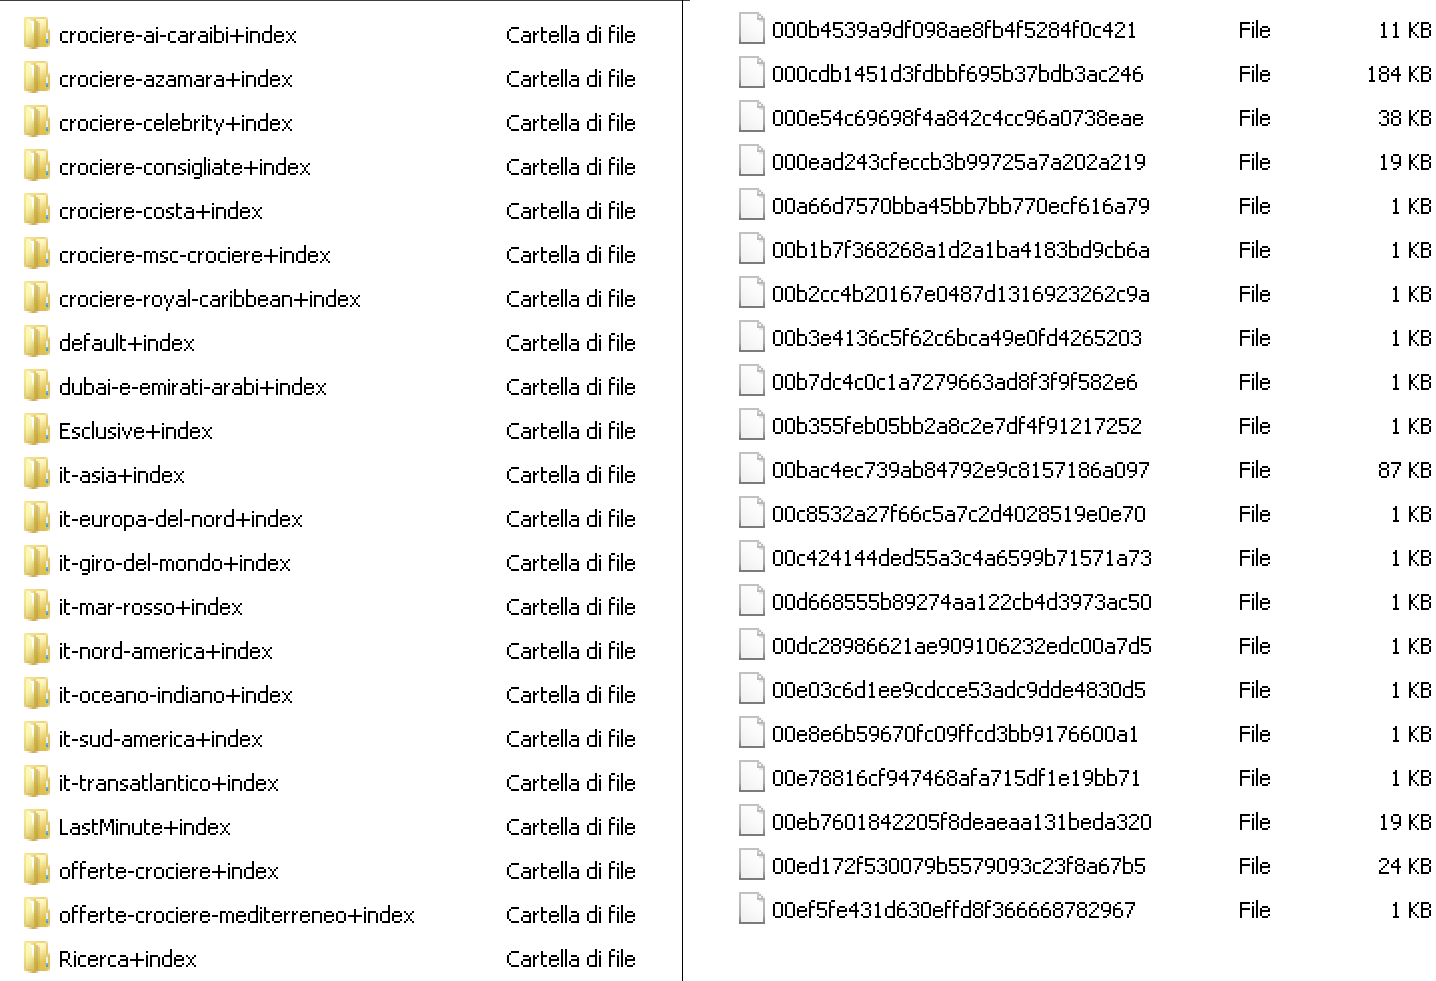
\includegraphics[width=1\columnwidth]{attivita/cache_codeigniter} 
	\caption{Struttura di cartelle e file di cache in esse contenuti.}
	\label{figura:cache-cartelle}
\end{figure}
\\
Grazie a \textit{cache\_delete} sarebbe possibile cancellare la cache solo di alcune pagine, ma è stato preferito non utilizzare tale funzione in quanto avrebbe aumentato inutilmente la complessità della soluzione.

\subsection{Risultati}
L'implementazione della cache ha giovato molto al \bookingEngine. Basti pensare che ora la pagina di visualizzazione dei risultati ricerca è giunta ad avere un tempo di risposta medio attorno ai 3 secondi, ovvero ora è l'80\% più veloce di prima, ma soprattutto è paragonabile al tempo di risposta dei competitor. Il tempo di risposta della homepage, inoltre, è arrivata a toccare i 500 millisecondi, dai circa 3 secondi prima di implementare la cache.\\
Tra ottimizzazione del database e cache, comunque, sono stati fatti ingenti miglioramenti alle prestazioni, che riassumo nella tabella \ref{table:risultati-ottimizzazioni}, prendendo come esempio la pagina principale e quella di visualizzazione dei risultati della ricerca (che, per brevità, chiamerò soltanto "ricerca").\\

\begin{table}[!h]
	\def\arraystretch{1.5}
	\begin{tabular}{ | l | l | l | l |}
		\hline
		\textbf{Pagina} & \textbf{Senza ottimizzazioni} & \textbf{Con DB ottimizzato} & \textbf{Con cache} \\ \hline
		Homepage & 7 secondi & 3 secondi & 0.5 secondi.  \\
		\hline
		Ricerca & 45-60 secondi & 15-20 secondi & 3 secondi.  \\
		\hline
	\end{tabular}
	\caption{Risultati delle ottimizzazioni effettuate sul \bookingEngine}
	\label{table:risultati-ottimizzazioni}
\end{table}


\newpage
\section{Integrazione delle tariffe \textit{vuoto per pieno}}
\subsection{Analisi del problema}
Dopo aver preso effettivamente confidenza con il database, mi è stato chiesto di creare un sistema che permettesse di inserire nel flusso di prenotazione anche tariffe \textit{vuoto per pieno}. Precisamente, tale sistema avrebbe dovuto avere le seguenti caratteristiche:
\begin{enumerate}
	\item Permettere di inserire nel sistema gli acquisti di \textit{vuoto per pieno} effettuati da \textit{Primarete} tramite upload di appositi file;
	\item Permettere di differenziare i prezzi in base al soggetto a cui si sta vendendo;
	\item Permettere di prenotare e pagare una cabina con tariffa \textit{vuoto per pieno}.
\end{enumerate}

\subsubsection{Inserimento degli acquisti nel sistema}
Il sistema deve prevedere una funzionalità di "carico" delle tariffe. In fase di acquisto di \textit{vuoto per pieno} da parte di \textit{Primarete}, il fornitore (ovvero la compagnia di crociera) rilascia un file riepilogativo contenente il dettaglio di quanto acquistato. Tali informazioni devono potersi caricare in modo assistito nel sistema, che avrebbe dovuto poi inserirle nel flusso di prenotazione.\\
Il problema principale è stato che il file ritornato da ciascun fornitore aveva (e ha tuttora) il proprio formato dati, quindi si sarebbe dovuto creare un importatore per ogni fornitore. Inoltre, anche la tipologia di dati presente in ciascun file poteva differire: ad esempio, per riferirsi all'età di ogni passeggero, alcuni fornitori utilizzano l'età ed altri la data di nascita. Il sistema avrebbe dunque dovuto uniformare i dati caricati.

\subsubsection{Differenziazione dei prezzi}
CrociereRegalo è un \bookingEngine\hphantom{i}utilizzato per vendite sia B2C (cioè verso clienti finali) sia B2B (cioè verso altre agenzie). Queste ultime, in base agli accordi commerciali che hanno con \textit{Primarete}, appartengono a determinati \textit{listini}, ovvero hanno diritto a commissioni/tariffe più o meno agevolate.\\Il sistema, quindi, avrebbe dovuto poter differenziare i prezzi di vendita delle cabine in base al listino di appartenenza dell'acquirente (un acquirente non appartenente a nessun listino sarebbe stato identificato al pari di una vendita B2C).

\subsubsection{Inserimento della tariffa nel flusso di prenotazione}
Il \bookingEngine\hphantom{i}avrebbe dovuto permettere di visualizzare i prezzi delle cabine soggette a tariffe \textit{vuoto per pieno} nei risultati di ricerca. Inoltre, avrebbe dovuto essere possibile poter prenotare e conseguentemente pagare tali cabine.\\La disponibilità delle stesse, quindi, si sarebbe dovuta aggiornare (decrementare) automaticamente.

\subsection{Progettazione e codifica della soluzione}
\subsubsection{Inserimento degli acquisti nel sistema - Progettazione}
Affinché fosse possibile inserire gli acquisti nel sistema, si è progettato di realizzare una nuova pagina riepilogativa nel pannello di amministrazione del \bookingEngine, accessibile solo tramite l'inserimento di username e password. In tale pagina viene visualizzato un riepilogo dei \textit{vuoto per pieno} caricati con la possibilità, per ognuno di essi, di avere il dettaglio delle cabine vendute e di quelle ancora disponibili. È stato inoltre inserito un tasto che apre una finestra di dialogo all'interno della quale viene data la possibilità di caricare nuovi \textit{vuoto per pieno}, andando quindi a "rifornire" il "magazzino". In base al fornitore selezionato nella finestra di dialogo è possibile: 
\begin{itemize}
	\item Caricare il file di riepilogo di quanto acquistato fornito dalla compagnia, in caso di fornitore \textbf{Costa} o \textbf{MSC}, come mostrato in Figura \ref{figura:upload-msc-costa}. Il primo fornisce un file con estensione \textit{.xls} mentre il secondo un file con estensione \textit{.csv}
	\begin{figure}[!h] 
		\centering 
		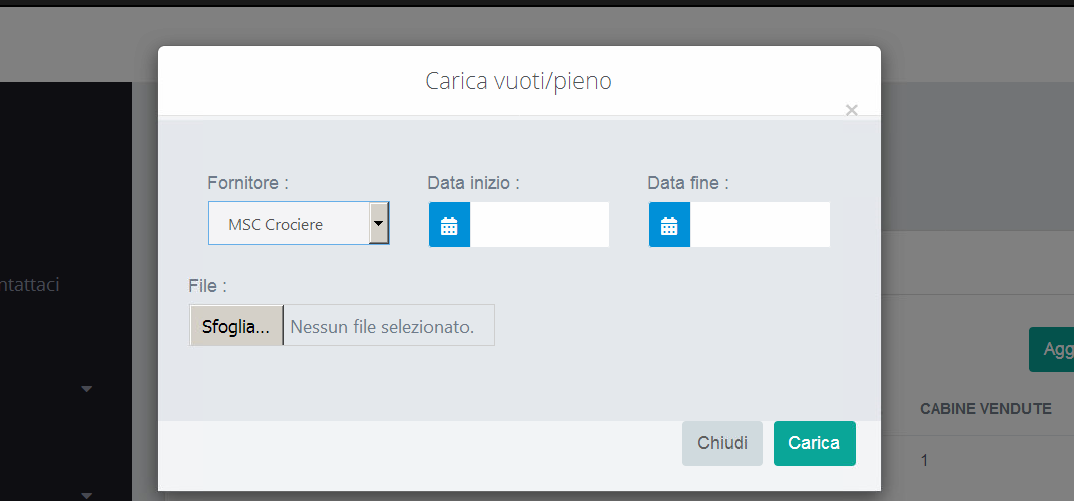
\includegraphics[width=.8\columnwidth]{attivita/vuotopieno_msc} 
		\caption{Schermata di caricamento del vuoto pieno MSC e Costa.}
		\label{figura:upload-msc-costa}
	\end{figure}
	\item Inserire a mano i dettagli del \textit{vuoto per pieno} che si intende caricare nel caso di fornitore \textbf{Royal Caribbean}, \textbf{Celebrity} o \textbf{Azamara}, come mostrato in Figura \ref{figura:upload-royal}. Essi infatti forniscono il file di riepilogo di quanto acquistato in formato \textit{.pdf}, che è molto difficile da interpretare.
	\begin{figure}[!h] 
		\centering 
		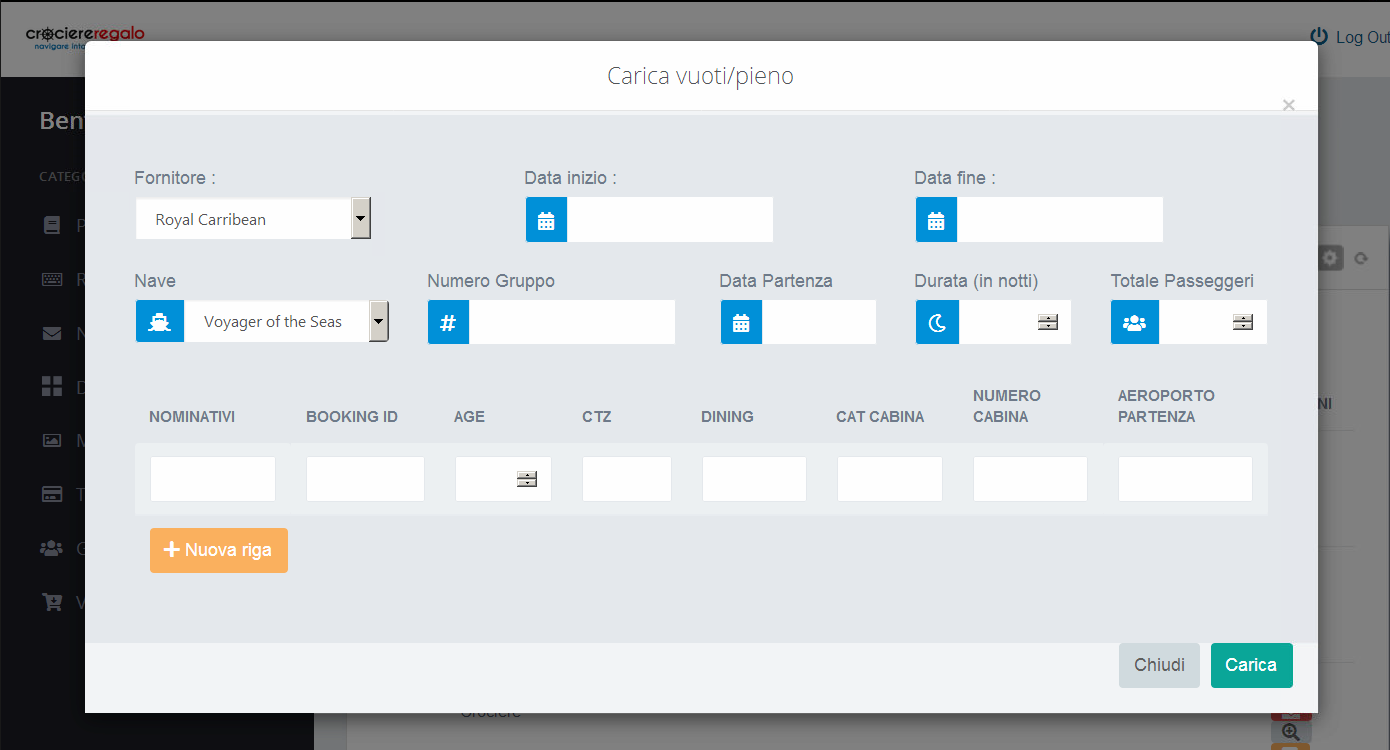
\includegraphics[width=.8\columnwidth]{attivita/vuotopieno_royal} 
		\caption{Schermata di caricamento del \textit{vuoto per pieno} Royal/Celebrity/Azamara.}
		\label{figura:upload-royal}
	\end{figure}
\end{itemize}
In ogni caso, è stato deciso che per ciascun \textit{vuoto per pieno} si sarebbero memorizzate le seguenti informazioni:
\begin{itemize}
	\item Il \textbf{fornitore}, ovvero MSC, Costa, Royal Caribbean, Celebrity o Azamara;
	\item Il \textbf{groupID}, ovvero un identificatore univoco per ciascun fornitore del \textit{vuoto per pieno} acquistato;
	\item Il \textbf{cruiseID}, ovvero un identificatore univoco per ciascun fornitore della crociera a cui tale \textit{vuoto per pieno} si riferisce;
	\item La \textbf{data di partenza} della crociera;
	\item La \textbf{lunghezza} (in numero di notti) della crociera;
	\item Il \textbf{numero di posti} (ovvero la capienza massima di persone) totali in quel \textit{vuoto per pieno};
	\item Il \textbf{numero di cabine} totali di quel \textit{vuoto per pieno},
	\item La \textbf{data di inizio} e la \textbf{data di fine} validità della tariffa, in modo che sia possibile venderla solo in determinati periodi/intervalli. Ciò significa che, ad esempio, se la data di inizio viene impostata al 20 agosto 2018 e la data di fine al 30 settembre 2018, in caso di una ricerca fatta prima del 20 agosto 2018 o dopo il 30 settembre 2018, la tariffa non comparirà tra i risultati.
\end{itemize}
\subsubsection{Inserimento degli acquisti nel sistema - Codifica}
Oltre alla realizzazione della pagina riepilogativa precedentemente progettata, per memorizzare queste informazioni è stata creata una nuova tabella in database denominata \textbf{Cruises\_Inventory}, avente come campi \textit{Id} (chiave primaria auto incrementante), \textit{Supplier} (fornitore, chiave esterna che si riferisce a \textit{Cruises\_Lines}, tabella dove sono memorizzati tutti i fornitori), \textit{GroupID}, \textit{CruiseID}, \textit{DepartureDate} (data di partenza della crociera), \textit{Length} (lunghezza in notti della crociera), \textit{N\_Pax} (numero di posti totali), \textit{N\_Cab} (numero di cabine totali), \textit{Data\_Inizio} e \textit{Data\_Fine}.\\
\\
Oltre alle informazioni generali relative a ciascun \textit{vuoto per pieno}, è stato necessario memorizzarne anche il contenuto in dettaglio, in termini di cabine acquistate (e quindi da rivendere). Si è deciso di creare la tabella \textbf{Cruises\_InventoryDetail} avente i seguenti campi:
\begin{itemize}
	\item \textbf{Id}, chiave primaria auto incrementante;
	\item \textbf{Cruises\_Inventory}, chiave esterna collegata all'\textit{Id} dell'omonima tabella \textit{Cruises\_Inventory}, che serve per collegare ogni riga del dettaglio al \textit{vuoto per pieno} corrispondente;
	\item \textbf{Cruises\_PricesID}, chiave esterna collegata all'\textit{Id} di \textit{Cruises\_Prices}, tabella il cui scopo verrà analizzato nel dettaglio nella sezione successiva;
	\item \textbf{Cabin}, numero di cabina (univoco nel dominio del fornitore) a cui la riga corrente fa riferimento;
	\item \textbf{BookId}, numero di prenotazione del fornitore della cabina a cui la riga corrente fa riferimento;
	\item \textbf{Category}, categoria della cabina corrente.
\end{itemize}
Per gestire il caricamento dei \textit{vuoto per pieno} nel sistema sono state realizzate tre classi \textit{parser} (una per MSC, una per Costa e una per il trio Royal-Celebrity-Azamara)in grado di interpretare dei dati in input e renderli compatibili con la struttura delle tabelle \textit{Cruises\_Inventory} e \textit{Cruises\_InventoryDetail}. Queste tre classi, \textit{MSCParser}, \textit{CostaParser} e \textit{RoyalParser} implementano tutte l'interfaccia \textbf{ParserInterface}, che ha i seguenti metodi astratti:
\begin{center}
	\def\arraystretch{1.5}
	\begin{tabularx}{\columnwidth}{XX}
		\hline
		\textbf{Metodo} & \textbf{Descrizione} \\ \hline
		+ getCruiseID() : string & Ritorna il CruiseID corrispondente al \textit{vuoto per pieno} considerato\\
		\hline
		+ getGroupID() : string & Ritorna il GroupID corrispondente al \textit{vuoto per pieno} considerato\\
		\hline
		+ getDepartureDate() : string & Ritorna la data di partenza corrispondente al \textit{vuoto per pieno} considerato, in formato "Y-m-d" (esempio 2018-09-27).\\
		\hline
		+ getLength() : int & Ritorna la lunghezza (in numero di notti) corrispondente al \textit{vuoto per pieno} considerato.\\
		\hline
		+ getNPax() : int & Ritorna la capienza totale (in numero di persone) corrispondente al \textit{vuoto per pieno} considerato.\\
		\hline
		+ getNCab() : int & Ritorna la capienza totale (in numero di cabine) corrispondente al \textit{vuoto per pieno} considerato.\\
		\hline
		+ popolaDettaglioTabella() : array & Ritorna un array che, per ciascuna riga del \textit{vuoto per pieno}, associa a ciascun campo della tabella \textit{Cruises\_InventoryDetail} il relativo valore.\\
		\hline
	\end{tabularx}
\end{center}
È stata poi creata una nuova classe, \textbf{Cruises\_Inventory}, derivata da \textit{CI\_Model} (classe base dei modelli di Codeigniter), che si occupa principalmente del caricamento del \textit{vuoto per pieno} nel database, avvalendosi dei parser prima elencati. Più precisamente, la classe ha i seguenti metodi:
\begin{center}
	\def\arraystretch{1.5}
	\begin{longtable}{ >{\raggedright}p{5.5cm} p{6.8cm}} 
		\hline
		\textbf{Metodo} & \textbf{Descrizione} \\ \hline
		+ validId(id:int) : boolean & Ritorna \textit{true} se il parametro passato è un valore presente nella colonna "Id" della tabella \textit{Cruises\_Inventory}\\
		\hline
		+ loadFromFile (supplier: int, fileContent: string, dataInizio: Date, dataFine: Date) : void & In base al fornitore passato come parametro (\textit{supplier}), carica il contenuto del \textit{vuoto per pieno} (presente in \textit{fileContent}) nel database, avvalendosi del parser associato al fornitore.\\
		\hline
		- loadRoyalInput (supplier: int, content: array) : boolean & Carica il \textit{vuoto per pieno} Royal/Celebrity/Azamara (in base al valore della variabile \textit{supplier}) leggendo il contenuto dall'array associativo \textit{content} ed elaborandolo grazie al parser \textit{RoyalParser}.\\
		\hline
		- loadCostaFile (fileContent: string) : boolean & Carica il \textit{vuoto per pieno} Costa nel database; \textit{fileContent} rappresenta il contenuto del file del \textit{vuoto per pieno} caricato, che verrà elaborato dal parser \textit{CostaParser}.\\
		\hline
		- loadMSCFile (fileContent: string) : boolean & Carica il \textit{vuoto per pieno} MSC nel database; \textit{fileContent} rappresenta il contenuto del file del \textit{vuoto per pieno} caricato, che verrà elaborato dal parser \textit{MSCParser}.\\
		\hline
		- saveParsedFile(parser: ParserInterface, supplier: int) : boolean & Metodo che viene chiamato da \textit{loadRoyalInput}, \textit{loadCostaFile}, \textit{loadMSCFile}; serve a popolare la tabella \textit{Cruises\_InventoryDetail} e la tabella \textit{Cruises\_Prices}.\\
		\hline
	\end{longtable}
\end{center}
La gestione del pannello di amministrazione è affidata ad un unico \textit{controller}, chiamato \textbf{Back}. In questa classe è stato aggiunto un metodo chiamato \textit{caricaVuotoPieno} che prende l'input dal frontend e lo passa al metodo \textit{loadFromFile} della classe \textit{Cruises\_Inventory} appena descritta, che si occuperà dell'elaborazione e della restituzione del risultato della stessa sotto forma di \gls{json}.

\subsubsection{Differenziazione dei prezzi - Progettazione}
I prezzi di ogni cabina presente nel sistema risiedono nella tabella \textit{Cruises\_Prices}. Tale tabella permette di conoscere il prezzo di ogni categoria di cabina (per ogni combinazione di età dei passeggeri tollerata dal sistema) per ogni \gls{tariffa} disponibile. Il problema è che \textit{Cruises\_Prices} viene svuotata e ripopolata ad ogni integrazione: per questo motivo si è deciso di separare la gestione dei prezzi delle cabine soggette a tariffa \textit{vuoto per pieno} in una nuova tabella, che è stata chiamata \textit{Cruises\_InventoryPrices}. 
\subsubsection{Differenziazione dei prezzi - Codifica}
Per realizzare quanto progettato, sono stati fatti i seguenti interventi:
\begin{itemize}
	\item Nella tabella \textit{Cruises\_Prices} è stata inserita una nuova colonna di tipo intero, \textbf{Manuale}, che indica se la riga si sta riferendo ad una tariffa passata dal fornitore o presa da un \textit{vuoto per pieno}. Quando viene fatta un'integrazione, vengono eliminate solo le righe aventi valore di tale colonna pari a 0, in modo da non perdere le informazioni relative al \textit{vuoto per pieno};
	\item È stata creata la tabella \textbf{Cruises\_InventoryPrices}, avente i seguenti campi:
		\begin{itemize}
			\item \textit{Id}, identificatore univoco della riga;
			\item \textit{Cruises\_Inventory}, chiave esterna che si riferisce al campo \textit{Id} di \textit{Cruises\_Inventory} e specifica il \textit{vuoto per pieno} di appartenenza di tale riga;
			\item \textit{Listino}, chiave esterna di \textit{Cruises\_Listini}, tabella appena creata che verrà descrittà nel prossimo paragrafo. In caso di valori NULL, il listino si intende essere \textit{B2C}, ovvero vendita al dettaglio;
			\item \textit{Categoria}, che rappresenta la categoria della cabina a cui ci si sta riferendo;
			\item \textit{Cabina}, che rappresenta il numero di cabina a cui ci si sta riferendo;
			\item \textit{BookId}, che indica il codice di prenotazione del fornitore collegato alla cabina a cui ci si sta riferendo;
			\item Un campo per ogni combinazione di prezzi tollerata dal sistema, ovvero \textit{Price1Adult, Price2Adult, Price3Adult, Price4Adult, Price1Adult1Junior, Price1Adult1Junior1Child, Price2Adult1Child, Price2Adult2Child, \\Price2Adult1Junior, Price2Adult2Junior, Price2Adult1Junior1Child};
			\item \textit{Commissione}, che quantifica la commissione spettante all'agenzia viaggi collegata al listino specificato, in caso il campo \textit{Listino} non sia NULL.
		\end{itemize}
\end{itemize}
La tabella \textbf{Cruises\_Listini} menzionata precedentemente è stata creata per poter gestire tutti i listini da collegare alle varie agenzie viaggi. Tale tabella presenta due campi, \textit{Id} e \textit{Nome}, usati appunto per definire il listino stesso. \\
Nella tabella \textit{Cruises\_Utenti}, che raccoglie tutte le agenzie viaggio che possono accedere alla modalità di acquisto B2B, è stato aggiunto il campo \textit{Listino}, chiave esterna di \textit{Cruises\_Listini}, in modo da associare ogni agenzia registrata ad un listino, in base agli accordi presi con \textit{Primarete}. \\ \\
Per l'interazione con la tabella \textit{Cruises\_InventoryPrices} è stato creato un nuovo model avente lo stesso nome della tabella, con i seguenti metodi: 
\begin{center}
	\def\arraystretch{1.5}
	\begin{longtable}{ >{\raggedright}p{5.5cm} p{6.8cm}} 
		\hline
		\textbf{Metodo} & \textbf{Descrizione} \\ \hline
		+ getColonnePrezzi() : array & Ritorna un array contentente la lista di tutte le combinazioni di prezzi tollerate dal sistema. Questo metodo è stato scritto per rendere poi dinamico l'inserimento dei prezzi in questa tabella, ovvero in caso si voglia aggiungere un nuovo campo non presente (ad esempio \textit{Price6Adult}), sarà sufficiente aggiungerlo come colonna della tabella, e interfaccia grafica e query di inserimento si adatteranno automaticamente. \\
		\hline
		+ tentaAggiornamentoPrezzi (tabella: array, inventoryId: int) : void & Metodo che prova ad aggiornare i prezzi nel caso di caricamento di un \textit{vuoto per pieno} contenente cabine già presenti nel sistema.\\
		\hline
		+ salvaPrezzi (input: array) : boolean & Metodo che salva i prezzi di ogni cabina, per ogni listino, presenti nel parametro \textit{input}. Ritorna \textit{true} in caso di successo, \textit{false} altrimenti.\\
		\hline
		+ modificaPrezzi (input: array) : boolean & Metodo che modifica i prezzi di ogni cabina, per ogni listino, presenti nel parametro \textit{input}. Ritorna \textit{true} in caso di successo, \textit{false} altrimenti.\\
		\hline
	\end{longtable}
\end{center}
È stato inoltre creato un metodo \textit{salvaPrezzi} nel controller \textit{Back}, che si limita ad invocare il metodo \textit{salvaPrezzi} del model \textit{Cruises\_InventoryPrices} con i parametri passati tramite POST.\\
A livello frontend, si è fatto in modo che, al termine del caricamento del \textit{vuoto per pieno}, si venga reindirizzati ad una pagina di inserimento prezzi (come quella mostrata in Figura \ref{figura:inserimento-prezzi-vuotopieno}), che permette appunto di specificare ogni combinazione di prezzo tollerata dal sistema per ogni categoria di cabina per ciascun listino. 
\begin{figure}[!h] 
	\centering 
	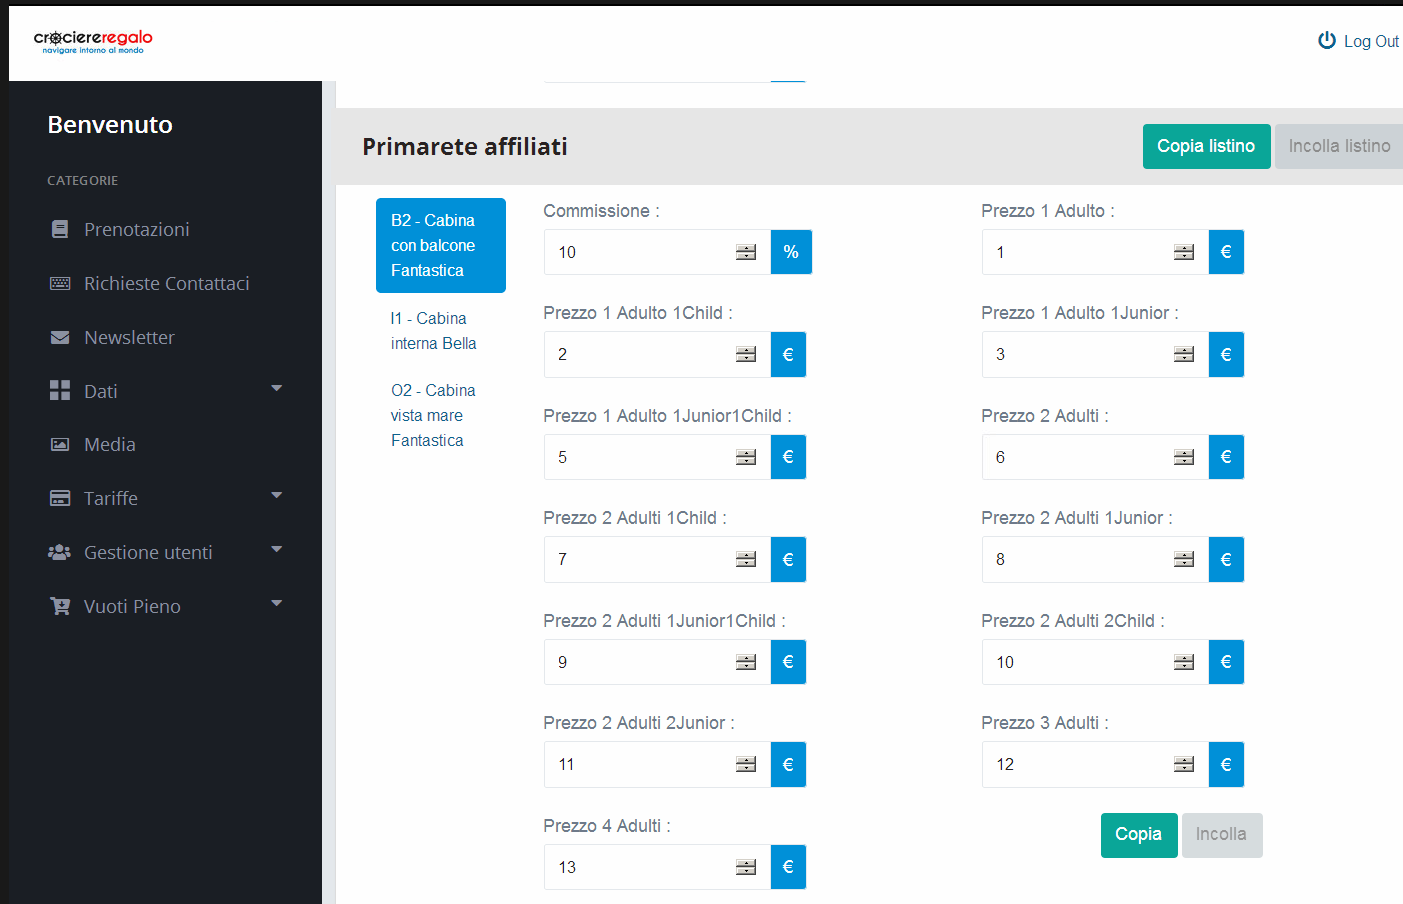
\includegraphics[width=1\columnwidth]{attivita/vuotopieno_prezzi} 
	\caption{Schermata di inserimento dei prezzi di un \textit{vuoto per pieno}.}
	\label{figura:inserimento-prezzi-vuotopieno}
\end{figure}\\
I prezzi poi vengono salvati tramite una chiamata \gls{ajax} che invoca il metodo \textit{salvaPrezzi} del controller \textit{Back} precedentemente descritto.

\subsubsection{Inserimento della tariffa nel flusso di prenotazione - Progettazione}
Come già accennato nella \hyperref[section:flusso-prenotazione]{Sezione \ref*{section:flusso-prenotazione}}, il flusso di prenotazione si compone di 6 step, a ciascuno dei quali corrisponde un metodo nel controller \textbf{WS\_Cruises} del \textit{dataExchange}. Questi 6 metodi venivano (e vengono tuttora) chiamati tramite richieste \gls{ajax} dal frontend e al loro interno chiamavano l'omologo metodo in grado di interfacciarsi con i \gls{webservice} del fornitore considerato. Si è deciso quindi di creare 6 nuovi metodi, uno per ogni step del flusso che, invece di interfacciarsi con qualche \gls{webservice}, leggesse i dati delle tariffe \textit{vuoto per pieno} direttamente dal database.\\
\subsubsection{Inserimento della tariffa nel flusso di prenotazione - Codifica}
Sono stati quindi creati i seguenti metodi:
\begin{center}
	\def\arraystretch{1.5}
	\begin{longtable}{ >{\raggedright}p{5.5cm} p{6.8cm}} 
		\hline
		\textbf{Metodo} & \textbf{Descrizione} \\ \hline
		+ Inventory\_categoryAvailabilty (inout wsResult:array) : void & Concatena al risultato eventualmente restituito dai \gls{webservice} del fornitore le categorie di cabine, se presenti, aventi tariffa \textit{vuoto per pieno}. Il codice della tariffa restituita (dato che servirà alle successive funzioni) è "INVENTORY".\\
		\hline
		+ Inventory\_cabinAvailabilty () : array & Legge dal database (facendo delle query su Cruises\_Inventory, Cruises\_InventoryDetail e Cruises\_InventoryPrices) e restituisce le singole cabine disponibili, compreso il prezzo, secondo i qualificatori che legge dal \textit{payload} della richiesta, quali numero ed età dei passeggeri, cruiseID considerato, categoria delle cabine di cui si vuole controllare la disponibilità e listino di appartenenza dell'utente.\\
		\hline
		+ Inventory\_requestPricing () : array & Calcola un preventivo in base ai parametri passati nel \textit{payload} della richiesta, ovvero fornitore, cruiseID, numero della cabina, dati anagrafici dei passeggeri.\\
		\hline
		+ Inventory\_requestBooking () : string & Prenota la cabina passata come parametro nel \textit{payload} della richiesta e ritorna il bookingID (identificativo della prenotazione) corrispondente.\\
		\hline
		+ Inventory \_requestBookingInformation (bookId: string) : array & Dato il bookId passato come parametro, restituisce tutti i dettagli inerenti alla prenotazione. \\
		\hline
	\end{longtable}
\end{center}
Il primo metodo del flusso, \textit{categoryAvailability}, in base al valore del parametro \textit{supplier} (letto dal \textit{payload} della richiesta), invocava i metodi \textit{MSC\_categoryAvailability} o \textit{Costa\_categoryAvailability}, che interrogano i rispettivi \glspl{webservice}. È stato sufficiente quindi che il nuovo metodo creato \textit{Inventory\_categoryAvailabilty} venisse invocato da \textit{categoryAvailabilty} a prescindere dal \textit{supplier}, concatenando all'output dei metodi \textit{MSC\_categoryAvailability} o \textit{Costa\_categoryAvailability} le categorie di cabine eventualmente disponibili con tariffa \textit{vuoto per pieno}.\\
Nei metodi \textit{cabinAvailability}, \textit{requestPricing}, \textit{requestBooking} e \textit{requestBookingInformation}, è stata introdotta un'istruzione condizionale che, in base al \textbf{fareCode} (codice della tariffa) passato come parametro, decide se invocare l'omologo metodo che legga dal database delle tariffe \textit{vuoto per pieno} (in caso di fareCode = "INVENTORY") o dai \glspl{webservice} del fornitore.\\
Al frontend, infine, non è stato necessario fare alcuna modifica.
\subsection{Test}
Al termine della realizzazione, sono stati effettuati test manuali sulla congruenza dei dati tra le nuove tabelle ed i \textit{vuoto per pieno} importati. Nello specifico:
\begin{itemize}
	\item Per i \textit{vuoto per pieno} \textbf{MSC} e \textbf{Costa}, si è verificato che il file venisse correttamente importato, interpretato e salvato nelle nuove tabelle realizzate \textit{Cruises\_Inventory} e \textit{Cruises\_InventoryDetail};
	\item Per i \textit{vuoto per pieno} \textbf{Royal}, \textbf{Celebrity} e \textbf{Azamara} si è verificato che la schermata di caricamento funzionasse e i dati venissero correttamente salvati nelle tabelle \textit{Cruises\_Inventory} e \textit{Cruises\_InventoryDetail}.
\end{itemize} 
Infine si è verificato che i dati presenti nelle tabelle fossero interpretati in maniera adeguata dalle varie query presenti nel flusso di prenotazione, dal primo all'ultimo dei sei step. Nello specifico: 
\begin{itemize}
	\item Si è verificato che il metodo \textbf{Inventory\_categoryAvailabilty} restituisse correttamente le categorie di cabine di un \textit{vuoto per pieno} preventivamente importato;
	\item Si è verificato che il metodo \textbf{Inventory\_cabinAvailabilty} restituisse correttamente le cabine di un \textit{vuoto per pieno} preventivamente importato;
	\item Si è verificato che il metodo \textbf{Inventory\_requestPricing} restituisse un preventivo corretto per una cabina disponibile di un \textit{vuoto per pieno} preventivamente importato, tenendo conto correttamente dei qualificatori passati (come l'età dei passeggeri);
	\item Si è verificato che il metodo \textbf{Inventory\_requestBooking} effettuasse e salvasse correttamente una nuova prenotazione a database, restituendone il codice corretto;
	\item Si è verificato che il metodo \textbf{Inventory\_requestBookingInformation} restituisse i dettagli corretti di un \textit{vuoto per pieno} preventivamente prenotato, in base a quanto presente nel database.
\end{itemize}
\newpage
\section{Aggiunta delle tariffe di un nuovo fornitore}
\subsection{Analisi del problema}
L'ultimo argomento affrontato durante lo stage è stato aggiungere la possibilità di prenotare una crociera con \textit{Royal Caribbean}, \textit{Celebrity} e \textit{Azamara}. Queste tre compagnie forniscono, grazie alla società \textit{ISTINFOR}, dei \glspl{webservice} chiamati \textbf{FIBOS}, che sono unici per le tre compagnie di crociera sopra citate. \\
\textit{FIBOS} prevede l'utilizzo di due tipologie di \glspl{webservice}: \textbf{FDF} (Fibos Data Feed) e \textbf{RCCL} (Royal Caribbean Cruise Line).
\subsubsection{Importazione delle informazioni statiche}
Per potersi interfacciare con i \glspl{webservice}, è stato necessario aggiungere al \bookingEngine\hphantom{i}le informazioni (codici, descrizioni) di aree geografiche, navi, porti e categorie di cabine utilizzate da FIBOS. Queste informazioni sono considerate statiche in quanto non cambiano spesso: si possono verificare delle variazioni solo in caso di varo di una nuova nave e/o costruzione di un nuovo porto.

\subsubsection{Utilizzo di FDF}
Questi \glspl{webservice} sono progettati per il trasferimento di grandi quantità di dati e forniscono un sistema di ricerca di crociere (e relativi prezzi). Si sono quindi dimostrati adatti al meccanismo di integrazione schedulata presente nel \bookingEngine. È stato dunque necessario creare un sistema che interrogasse i \glspl{webservice} \textit{FDF}, consolidandone i risultati nel \textit{DataExchange} ed integrandoli poi nell'\textit{OTA}. 

\subsubsection{Utilizzo di RCCL}
Per far fronte ai dati richiesti in tempo reale dal flusso di prenotazione, invece, sono stati offerti da \textit{FIBOS} i \glspl{webservice} \textbf{RCCL}, che è stato necessario integrare ed interrogare.

\subsection{Progettazione e codifica della soluzione}
\subsubsection{Importazione delle informazioni statiche - Progettazione}
Informazioni circa codici di aree geografiche, navi, porti, categorie di cabine, ponti ci sono state fornite da \textit{ISTINFOR} in un file formato \textit{.xlsx}. In caso di variazioni di tali informazioni, per contratto, ci sarebbe stato mandato un nuovo file aggiornato. Proprio per questo è stato deciso, invece di importare a mano i dati, di realizzare un importatore.\\
A livello grafico, si è deciso di realizzare una semplice finestra di dialogo che permettesse di caricare il file in oggetto e mandarlo al backend per l'elaborazione. A livello backend, si è deciso di realizzare una nuova classe che gestisse l'importazione del file ed il suo corretto salvataggio nel database.

\subsubsection{Importazione delle informazioni statiche - Codifica}
A livello frontend, si è realizzata la finestra di dialogo descritta in precedenza. Il risultato è mostrato in Figura \ref{figura:upload-fibos}.
\begin{figure}[!h] 
	\centering 
	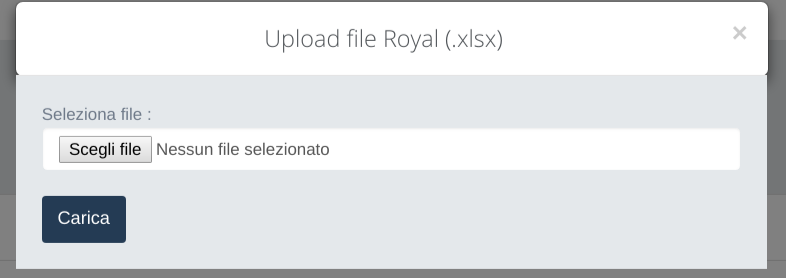
\includegraphics[width=.6\columnwidth]{attivita/upload_royal} 
	\caption{Schermata di caricamento del file passato da ISTINFOR}
	\label{figura:upload-fibos}
\end{figure} \\
A livello backend, per gestire l'importazione del file, è stato realizzato un nuovo model nella parte \textit{OTA}, chiamato semplicemente \textit{Royal}, avente i seguenti metodi:
\begin{center}
	\def\arraystretch{1.5}
	\begin{longtable}{ >{\raggedright}p{5.5cm} p{6.8cm}} 
		\hline
		\textbf{Metodo} & \textbf{Descrizione} \\ \hline
		+ parse(fileName: string) : boolean & Elabora il file avente nome (e percorso) 'fileName'. Restituisce true se l'elaborazione è andata a buon fine, false altrimenti .\\
		\hline
		- loadPorts () : boolean & Viene invocato da \textit{parse}, si occupa di leggere i porti dal file e caricarli nella tabella \textit{Cruises\_Ports} del \textit{DataExchange} (che poi viene sincronizzata, ad ogni integrazione, con l'omonima tabella dell'\textit{OTA}). Restitusce \textit{true} in caso di successo, \textit{false} altrimenti.\\
		\hline
		- loadShips () : boolean & Viene invocato da \textit{parse}, si occupa di leggere le navi dal file e caricarle nella tabella \textit{Cruises\_Ships} del \textit{DataExchange} (che poi viene sincronizzata, ad ogni integrazione, con l'omonima tabella dell'\textit{OTA}). Restitusce \textit{true} in caso di successo, \textit{false} altrimenti.\\
		\hline
		- loadDecks () : boolean & Viene invocato da \textit{parse}, si occupa di leggere i ponti delle varie navi dal file e caricarli nella tabella \textit{Cruises\_Decks} del \textit{DataExchange} (che poi viene sincronizzata, ad ogni integrazione, con l'omonima tabella dell'\textit{OTA}). Restitusce \textit{true} in caso di successo, \textit{false} altrimenti.\\
		\hline
		- loadCategories () : boolean & Viene invocato da \textit{parse}, si occupa di leggere le categorie di cabine delle varie navi dal file e caricarle nella tabella \textit{Cruises\_CabinCategories} del \textit{DataExchange} (che poi viene sincronizzata, ad ogni integrazione, con l'omonima tabella dell'\textit{OTA}). Restitusce \textit{true} in caso di successo, \textit{false} altrimenti.\\
		\hline
	\end{longtable}
\end{center}
È stato poi creato un nuovo metodo \textit{caricaRoyal} sul controller \textit{Back} dell'\textit{OTA}, che prende il file caricato dal frontend e lo passa al metodo \textit{parse} del model \textit{Royal} sopra descritto.

\subsubsection{Utilizzo di FDF - Progettazione}
Nel file \textit{.xlsx} fornito da \textit{ISTINFOR} mancano tutte le informazioni inerenti a itinerari, prezzi e partenze delle crociere. Queste sono invece fornite dal \gls{webservice} \textbf{FDF}, che quindi si è dovuto implementare. L'interazione con tale \gls{webservice} avviene tramite chiamate \gls{SOAP} ad appositi URL forniti da \textit{ISTINFOR}.\\ Essendoci stati forniti solo degli URL di sviluppo, le chiamate restituiscono dati verosimili ma non veri. Inoltre, \textit{ISTINFOR} utilizza un firewall: vengono accettate richieste provenienti solo da IP noti. Siccome il server di sviluppo utilizzato era all'interno della rete dell'ufficio, con IP dinamico e non esposto, è stato necessario creare un ambiente online di test, da affiancare a quello di produzione (all'indirizzo \cite{site:sviluppo-crociereregalo} e \cite{site:sviluppo-dataexchange}).\\
Premesso ciò, la struttura di una chiamata \gls{SOAP} accettata da \textit{FDF} è la seguente:
\begin{lstlisting}
<SOAP-ENV:Envelope xmlns:SOAP-ENV="http://schemas.xmlsoap.org/soap/envelope/" xmlns:ns1="http://tempuri.org/WebService/Service1">
  <SOAP-ENV:Body>
    <ns1:PROCEDURA>
      <ns1:MessageXML>
        <PROCEDURA>
          <Header>
            <CruiseLineCode>RCCL</CruiseLineCode>
            <SubsystemId>2</SubsystemId>
            <AgencyId1>041178383</AgencyId1>
            <AgencyId2>041178383</AgencyId2>
            <Currency>EUR</Currency>
            <AgencyConsumer>A</AgencyConsumer>
          </Header>
          <PROCEDURA>
            <PARAMETRO/>
          </PROCEDURA>
        </PROCEDURA>
      </ns1:MessageXML>
    </ns1:PROCEDURA>
  </SOAP-ENV:Body>
</SOAP-ENV:Envelope>
\end{lstlisting} 
Il tag \textit{Header} ed il suo contenuto sono comuni a tutte le richieste. Bisogna poi sostituire il nome \textit{PROCEDURA} con quello della funzione che si vuole invocare (ad esempio \textit{SearchBySea}) e, in base a quanto definito nella documentazione, includere una lista di parametri (allo stesso livello del tag \textit{Parametro}). Prima di invocare una procedura generica, però, è necessario fare una chiamata alla funzione di login, che permette di autenticarsi, come mostrato in Figura \ref{figura:flowchart-login-webservice}.
\begin{figure}[!h] 
	\centering 
	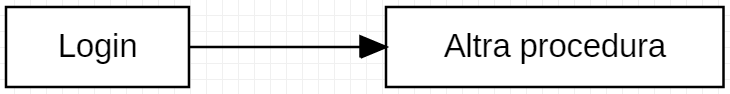
\includegraphics[width=.6\columnwidth]{attivita/flowchart-login-webservice} 
	\caption{Flow chart dell'invocazione di una qualsiasi procedura FDF.}
	\label{figura:flowchart-login-webservice}
\end{figure}\\
\subsubsection{Utilizzo di FDF - Codifica}
Tutte le chiamate ai \gls{webservice} vengono gestite dal \textit{DataExchange}, all'interno del quale sono state create due nuove classi per semplificarne l'interazione: \textit{Royal\_Model} e \textit{Royal\_WS}.\\
La prima è un model che serve ad effettuare le chiamate ai \gls{webservice} forniti, e si compone dei seguenti metodi:
\newpage
\begin{center}
	\def\arraystretch{1.5}
	\begin{longtable}{ >{\raggedright}p{5.5cm} p{6.8cm}} 
		\hline
		\textbf{Metodo} & \textbf{Descrizione} \\
		\hline
		- buildHeader(lineCode: string) : void & Costruisce e salva in una variabile interna alla classe l'intestazione della richiesta, popolando contenuto il tag \textit{<CruiseLineCode>} con il valore del parametro \textit{lineCode} passato.\\
		\hline
		- callWS (xml: string, function: string) : SimpleXMLObject & Fa una richiesta al \gls{webservice}, chiamando la procedura remota \textit{function}, utilizzando come \textit{payload} il valore del parametro \textit{xml}. Restituisce la risposta del \gls{webservice} come istanza di SimpleXMLObject (che permette di muoversi agevolmente tra i vari tag e attributi), oppure NULL in caso si verifichi un errore di parsing (ad esempio la risposta non sia in XML ben formattato).\\
		\hline
		+ login (lineCode: string) : boolean & Effettua la chiamata alla procedura remota di login, avvalendosi della funzione \textit{buildHeader}, alla quale viene passato il parametro \textit{lineCode}.\\
		\hline
		+ requestPricesSea (sea: string, date: string, guests: int) : SimpleXMLObject & Effettua una \gls{RPC} al metodo \textit{RequestSearchBySeaPricing} del \gls{webservice}, con i parametri \textit{Sea}, \textit{Date} e \textit{Guests} valorizzati in base a quanto passato.\\
		\hline
	\end{longtable}
\end{center}
Il metodo \textit{RequestSearchBySeaPricing} di \textit{FDF} permette di effettuare una ricerca del miglior prezzo per ogni categoria di cabina di tutte le partenze di tutte le navi gestite dal sistema (quindi Royal, Celebrity e Azamara). Nella ricerca possono essere inserite delle restrizioni sul numero di passeggeri, sull'area geografica (mare) di navigazione e su un intervallo di date (ad esempio crociere che partono dal 3 settembre 2018 al 10 ottobre 2019). \\
La chiamata a \textit{RequestSearchBySeaPricing} (quindi al metodo \textit{requestPricesSea} di \textit{Royal\_Model}) viene utilizzata dal meccanismo schedulato di integrazione per popolare le informazioni inerenti agli itinerari disponibili, alle date di partenza di ogni itinerario e ai prezzi di ogni categoria di cabina di ogni data di partenza di ogni itinerario. Tale elaborazione richiede molto tempo (fino a 40 minuti), per tanto viene eseguita durante la notte (è stato deciso di schedularla alle 2 del mattino, dato che non c'é un orario preciso di rilascio dei nuovi aggiornamenti). \\
Per permettere l'invocazione di tale metodo è stato realizzato un controller apposito, chiamato \textit{Royal\_WS}, il cui contenuto è il seguente:
\newpage
\begin{center}
	\def\arraystretch{1.5}
	\begin{longtable}{ >{\raggedright}p{5.5cm} p{6.8cm}} 
		\hline
		\textbf{Metodo} & \textbf{Descrizione} \\
		\hline
		+ load\_PricesSea() : void & Tramite la chiamata al metodo \textit{requestPricesSea} del model \textit{Royal\_Model}, sincronizza, per ogni itinerario, la lista delle partenze (incluse disponibilità di cabine, prezzi e in generale tutto quanto restituito dalla funzione) con il database del \textit{DataExchange}. Grazie al meccanismo dei \textit{magic method} descritto in sezione \ref{section:struttura-codice}, esso può essere invocato direttamente via URL.\\
		\hline
	\end{longtable}
\end{center}

\subsubsection{Utilizzo di RCCL - Progettazione}
Il metodo \textit{RequestSearchBySeaPricing} di \textit{FDF}, ai fini dell'integrazione dati, presentava un grande difetto: non restituiva il dettaglio dell'itinerario, ma vi si riferiva utilizzandone solo il codice. Ciò rappresentava un problema sia ai fini della ricerca offerta dal \bookingEngine\hphantom{i}che della visualizzazione dei dettagli di una crociera. In tale pagina, infatti, è presente la lista di destinazioni toccate dalla crociera, mostrata in Figura \ref{figura:destinazioni-crociera}. Per reperire queste informazioni si sarebbe potuto mappare a mano ciascun itinerario in base alle informazioni contenute nei cataloghi cartacei delle tre compagnie, ma sarebbe stato un lavoro enorme (gli itinerari sono circa 1400 in totale) che si sarebbe dovuto ripetere costantemente nel tempo, in quanto essi cambiano ogni manciata di mesi.\\
\begin{figure}[!h] 
	\centering 
	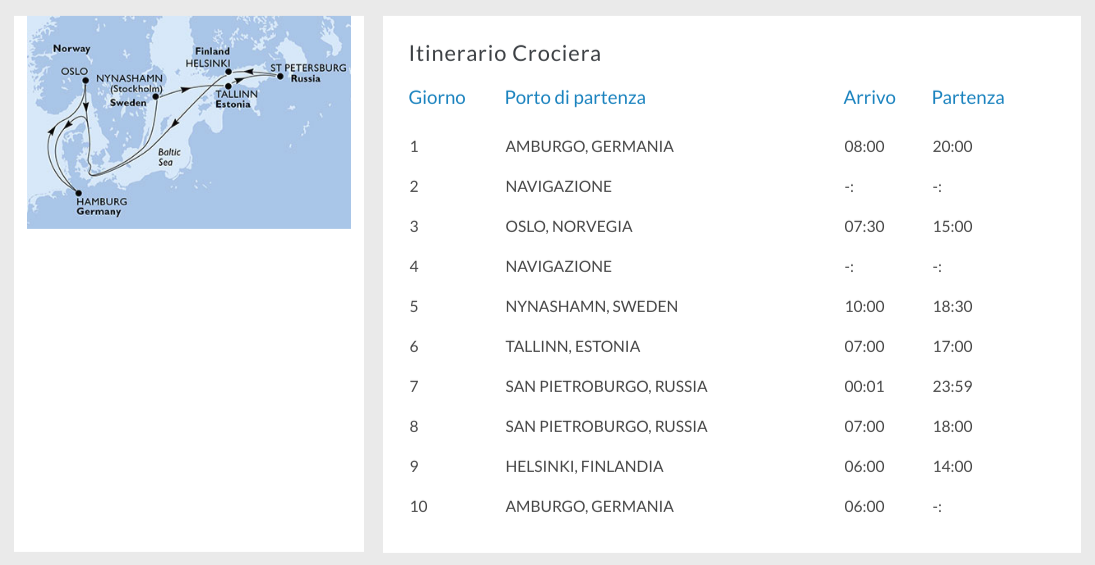
\includegraphics[width=.9\columnwidth]{attivita/dettaglio_itinerario} 
	\caption{Dettaglio dell'itinerario visualizzato dal frontend.}
	\label{figura:destinazioni-crociera}
\end{figure}\\ \\Per evitare tanto lavoro si è deciso di implementare, all'interno del metodo \textit{load\_PricesSea} della classe \textit{Royal\_WS}, delle \gls{RPC} a \textit{RequestItinerary}, fornito dal \gls{webservice} \textit{RCCL}, che restituisce le informazioni dettagliate dell'itinerario corrispondente ai parametri passati (codice della nave, data di partenza e codice itinerario).  Dato che il protocollo di comunicazione è analogo a quello utilizzato per \textit{FDF}, si è deciso (per questo e per tutti le altre \gls{RPC} utilizzate di \textit{RCCL}) di riutilizzare la classe \textit{Royal\_Model}, andando a definire nuovi metodi in base alle necessità. 

\subsubsection{Utilizzo di RCCL - Codifica}
In questo caso è stato aggiunto il seguente metodo: 
\begin{center}
	\def\arraystretch{1.5}
	\begin{longtable}{ >{\raggedright}p{5.5cm} p{6.8cm}} 
		\hline
		\textbf{Metodo} & \textbf{Descrizione} \\
		\hline
		+ requestItinerary(ship: string, date: string, itinerary: string) : SimpleXMLObject & Effettua una \gls{RPC} a \textit{RequestItinerary} del \gls{webservice}, con i parametri \textit{Ship}, \textit{Date} e \textit{Itinerary} valorizzati in base a quanto passato. Ritorna la risposta in forma di oggetto SimpleXMLObject, o NULL in caso di risposta mal formattata.\\
		\hline
	\end{longtable}
\end{center}
Le informazioni ritornate da questo metodo includono anche la lista di destinazioni dell'itinerario, ma la lingua in cui i nomi di tali destinazioni (porti, città, stati) vengono restituiti è mista. Ad esempio, per riferirsi alle isole delle Azzorre, viene usato tanto il nome italiano "Azzorre" quanto il nome spagnolo "Azores". La stessa cosa vale per Danimarca, Scozia, Australia, Emirati Arabi, Canarie, Belgio ecc. È stato dunque necessario realizzare un mapping manuale dei nomi, che permettesse di tradurre i nomi in lingua italiana.\\ \\
Per quanto riguarda l'integrazione nel flusso di prenotazione delle tariffe \textit{FIBOS}, analogamente al lavoro svolto per i \textit{vuoto per pieno}, sono stati creati ed implementati nuovi metodi nel controller \textit{WS\_Cruises} che utilizzano nuovi metodi creati nel model \textit{Royal\_Model}. Sono state utilizzate le seguenti procedure di \textit{RCCL}:

\begin{center}
	\def\arraystretch{1.5}
	\begin{longtable}{ >{\raggedright}p{5.5cm} p{6.8cm}} 
		\hline
		\textbf{Procedura} & \textbf{Descrizione} \\
		\hline
		RequestCategories & Dati in input nave (Ship), data di partenza (Date), numero ed età dei passeggeri (Guests), restituisce una lista di tariffe disponibili per quella partenza, complete di prezzi per ogni categoria di cabina, tasse portuali ed eventualmente oneri aggiuntivi.\\
		\hline
		RequestCabins &  Dati in input nave (Ship), data di partenza (Date), numero ed età dei passeggeri (Guests) e codice della tariffa (FareCode), restituisce una lista di cabine disponibili che soddisfano i criteri definiti dai parametri passati.\\
		\hline
		RequestPricing &  Dati in input nave (Ship), data di partenza (Date), numero ed età dei passeggeri (Guests), codice della tariffa (FareCode) e della cabina (Cabin), restituisce una quotazione veritiera che soddisfa i criteri definiti dai parametri passati.\\
		\hline
		RequestBooking &  Dati in input nave (Ship), data di partenza (Date), numero, età e dati anagrafici dei passeggeri (Guests), codice della tariffa (FareCode) e della cabina (Cabin) e la tipologia di prenotazione che si vuole effettuare (AgreementSt, da porre a OF in caso si voglia fare un'opzione, mentre a BK in caso di prenotazione vera e propria), restituisce il codice di prenotazione (BookingId), assieme all'ammontare di denaro e relative scadenze dei pagamenti.\\
		\hline
		RequestRetrieve &  Dato in input il numero di prenotazione (BookingId), restituisce le informazioni dettagliate (sia inerenti all'itinerario, sia allo stato dei pagamenti) della prenotazione corrispondente.\\
		\hline
	\end{longtable}
\end{center}
Per effettuare le \gls{RPC} sopra descritte, sono stati realizzati i seguenti nuovi metodi all'interno della classe \textit{Royal\_Model}:
\begin{center}
	\def\arraystretch{1.5}
	\begin{longtable}{ >{\raggedright}p{5.5cm} p{6.8cm}} 
		\hline
		\textbf{Metodo} & \textbf{Descrizione} \\
		\hline
		+ categoryAvailability(ship: string, date: string, guests: array) : SimpleXMLObject & Effettua una \gls{RPC} a \textit{RequestCategories} del \gls{webservice}, con i parametri \textit{Ship}, \textit{Date} e \textit{Guests} valorizzati in base a quanto passato. Ritorna la risposta in forma di oggetto SimpleXMLObject, o NULL in caso di risposta mal formattata.\\
		\hline
		+ cabinAvailability(ship: string, date: string, guests: array, fareCode: string) : SimpleXMLObject & Effettua una \gls{RPC} a \textit{RequestCabins} del \gls{webservice}, con i parametri \textit{Ship}, \textit{Date}, \textit{Guests}, \textit{FareCode} valorizzati in base a quanto passato. Ritorna la risposta in forma di oggetto SimpleXMLObject, o NULL in caso di risposta mal formattata.\\
		\hline
		+ pricingInformation(ship: string, date: string, cabin: string, fareCode: string, guest: array) : SimpleXMLObject & Effettua una \gls{RPC} a \textit{RequestPricing} del \gls{webservice}, con i parametri \textit{Ship}, \textit{Date}, \textit{Guests}, \textit{FareCode}, \textit{Cabin} valorizzati in base a quanto passato. Ritorna la risposta in forma di oggetto SimpleXMLObject, o NULL in caso di risposta mal formattata.\\
		\hline
		+ book(ship: string, date: string, cabin: string, fareCode: string, guest: array, agreementSt: string) : SimpleXMLObject & Effettua una \gls{RPC} a \textit{RequestBooking} del \gls{webservice}, con i parametri \textit{Ship}, \textit{Date}, \textit{Guests}, \textit{FareCode}, \textit{Cabin}, \textit{AgreementSt} valorizzati in base a quanto passato. Ritorna la risposta in forma di oggetto SimpleXMLObject, o NULL in caso di risposta mal formattata.\\
		\hline
		+ retrieveBooking(bookingNumber: string) : SimpleXMLObject & Effettua una \gls{RPC} a \textit{RequestRetrieve} del \gls{webservice}, con il parametro \textit{BookingId} valorizzato in base a quanto passato. Ritorna la risposta in forma di oggetto SimpleXMLObject, o NULL in caso di risposta mal formattata.\\
		\hline
	\end{longtable}
\end{center}
Infine, per invocare ed elaborare i risultati dei nuovi metodi scritti in \textit{Royal\_Model}, sono state aggiunte le seguenti funzioni a \textit{WS\_Cruises}:
\begin{center}
	\def\arraystretch{1.5}
	\begin{longtable}{ >{\raggedright}p{5.5cm} p{6.8cm}} 
		\hline
		\textbf{Metodo} & \textbf{Descrizione} \\
		\hline
		+ Fibos\_categoryAvailability (supplier: int, cruiseID: string, guest: array) : array & Restituisce un array contenente la lista delle categorie di cabina effettivamente disponibili, interrogando il \gls{webservice} tramite l'invocazione del metodo \textit{categoryAvailability} di \textit{Royal\_Model}.\\
		\hline
		+ Fibos\_cabinAvailability (supplier: int, cruiseID: string, guest: array, fareCode: string) : array & Restituisce un array contenente la lista delle singole cabina effettivamente disponibili, interrogando il \gls{webservice} tramite l'invocazione del metodo \textit{categoryAvailability} di \textit{Royal\_Model}, tenendo conto dei parametri passati (quindi anche del fareCode, ovvero della tariffa scelta allo step precedente).\\
		\hline
		+ Fibos\_requestPricing (supplier: int, cruiseID: string, guest: array, fareCode: string, cabin: string) : array & Restituisce un array contenente una quotazione veritiera per la cabina selezionata (tenendo conto di tariffa, crociera, cabina, selezionate e del numero ed età dei passeggeri), interrogando il \gls{webservice} tramite l'invocazione del metodo \textit{pricingInformation} di \textit{Royal\_Model}.\\
		\hline
		+ Fibos\_requestBooking (supplier: int, cruiseID: string, guest: array, fareCode: string, cabin: string, agreementSt: string) : array & Effettua una prenotazione in base ai parametri passati (tariffa, crociera, cabina, numero ed età dei passeggeri, tipo di prenotazione), interrogando il \gls{webservice} tramite l'invocazione del metodo \textit{book} di \textit{Royal\_Model}.\\
		\hline
		+ Fibos\_requestBookingInformation (bookingNumber: string) : array & Restituisce le informazioni inerenti alla prenotazione passata come parametro, interrogando il \gls{webservice} tramite l'invocazione del metodo \textit{retrieveBooking} di \textit{Royal\_Model}.\\
		\hline
	\end{longtable}
\end{center}

\subsubsection{Problemi riscontrati}
Nell'implementazione dei due \glspl{webservice} sopra menzionati, sono stati riscontrati dei problemi, principalmente con la documentazione fornitaci da \textit{ISTINFOR}. All'inizio, infatti, ci sono stati forniti i manuali aggiornati a febbraio 2014, e molti parametri delle procedure da noi usate non corrispondevano a quanto scritto nel manuale. Dopo numerose sollecitazioni, siamo riusciti ad ottenere la guida aggiornata all'ultima release (febbraio 2018).\\
Un altro problema riscontrato, forse quello che ci ha fatto perdere più tempo, è stato l'eterogeneità dei formati delle date richiesti dai parametri/tag/attributi delle varie procedure. Infatti, alcune di esse richiedevano che la data fosse espressa in formato YYYY-mm-dd (ovvero 2018-09-27), altre in formato YYYYmmdd (20180927), altre ancora in formato dd/mm/YYYYY (27/09/2018) o addirittura mm/dd/YYYY (09/27/2018). Al di là delle numerose conversioni necessarie per adattarle al formato presente nel database (che è YYYY-mm-dd), il problema è stato che il manuale si è rivelato ambiguo riguardo al formato corretto da usare (o non veniva specificato o, addirittura, veniva specificato un formato sbagliato). Visto anche l'elevato tempo di risposta (settimane) del supporto tecnico, soprattutto probabilmente perché lo stage si è svolto durante il periodo estivo tipico delle ferie, abbiamo dovuto procedere molto spesso per tentativi, perdendo molto tempo.

\subsection{Test}
Anche in questo caso, vista l'assenza di una suite di testing, si sono svolte delle verifiche a mano di congruenza tra i dati restituiti da i \gls{webservice} e quelli presenti nel database. Inoltre, grazie alle credenziali di accesso forniteci da \textit{Primarete}, è stato possibile verificare la congruenza tra quanto presente nel database e quanto visualizzato dal portale di prenotazione ufficiale del gruppo Royal/Celebrity/Azamara. I dati in nostro possesso, sebbene derivanti da canali di test e non di produzione, erano in pratica dati reali, solo semplicemente non aggiornati.